\documentclass{ieeeaccess}
\usepackage{cite}
\usepackage{amsmath,amssymb,amsfonts}
\usepackage{algorithmic}
\usepackage{graphicx}
\usepackage{textcomp}
\usepackage{url}
\usepackage{array}
\usepackage{multirow}
\usepackage{booktabs}
\usepackage{bm}

\def\BibTeX{{\rm B\kern-.05em{\sc i\kern-.025em b}\kern-.08em
    T\kern-.1667em\lower.7ex\hbox{E}\kern-.125emX}}

\begin{document}
\history{Date of publication March 00, 2026, date of current version March 00, 2026.}
\doi{10.1109/ACCESS.2026.DOI-PLACEHOLDER}

\title{ORCHESTRA: Emergent Organizational Evolution in Autonomous AI Agent Societies}

\author{\uppercase{First A. Author}\authorrefmark{1},
\uppercase{Second B. Author}\authorrefmark{2}, and
\uppercase{Third C. Author}\authorrefmark{3}, \IEEEmembership{Member, IEEE}}
\address[1]{Department of Computer Science and Engineering, Premier Research Institute, City, State, Country (e-mail: first.author@institute.edu)}
\address[2]{Department of Artificial Intelligence, Technological University, City, State, Country (e-mail: second.author@techuniv.edu)}
\address[3]{Department of Information Technology, National Research Center, City, State, Country (e-mail: third.author@research.org)}
\tfootnote{This research was supported in part by the National Science Foundation and the Advanced Multi-Agent Intelligence Research Initiative under Grant UROP-2026-ORCHESTRA. The authors gratefully acknowledge the computational resources and infrastructure support provided for experimental evaluation.}

\markboth
{Author \headeretal: ORCHESTRA: Emergent Organizational Evolution in Autonomous AI Agent Societies}
{Author \headeretal: ORCHESTRA: Emergent Organizational Evolution in Autonomous AI Agent Societies}

\corresp{Corresponding author: First A. Author (e-mail: first.author@institute.edu).}

\begin{abstract}
Contemporary multi-agent systems powered by large language models (LLMs) predominantly depend on human-engineered, rigid organizational structures---such as centralized star coordinators, static hierarchical trees, or unconstrained all-to-all broadcast debate. While effective for simple conversational workflows, these predetermined structures exhibit severe structural vulnerabilities: centralized coordinators become severe token and latency bottlenecks, static tree hierarchies collapse catastrophically when intermediate nodes fail, and unconstrained broadcast triggers quadratic message growth. In this paper, we introduce \textbf{ORCHESTRA}, a principled research framework for investigating emergent organizational evolution, behavioral specialization, and structural resilience in autonomous AI agent societies initialized with \textit{zero predefined roles} and \textit{unconstrained peer-to-peer communication}. Grounded in the standardized SILO-BENCH distributed coordination benchmark (ACL 2026), we conduct a rigorous empirical investigation encompassing 300 executed experimental runs across agent scales $N \in \{2, 5\}$ and 15 stratified algorithmic tasks spanning three complexity tiers (cross-silo aggregation, spatial mesh routing, and global shuffle algorithms), powered by the Qwen 3.8 27B foundation model. We benchmark ORCHESTRA against four canonical literature paradigms: Independent Ensembles (Wang et al., 2023), Flat Broadcast Debate (ChatDev; Qian et al., 2024), Central Star Coordinator (AutoGen; Wu et al., 2024), and Hierarchical Tree (MacNet; Wang et al., 2024). We introduce a quantitative metric suite combining economic inequality measures (Gini degree specialization $G$) and graph-theoretic dynamics (Jaccard structural drift $J$, reciprocity $R$, and betweenness centrality). Our empirical findings reveal the existence of an \textit{Emergence Curve}: agents initialized symmetrically autonomously transition from flat democratic coordination on simple tasks ($G=0.266$) to spontaneous leadership hub election on complex distributed algorithms ($G=0.401$) and dynamic organizational consolidation under node crash perturbations ($G=0.600$). On the most challenging Level~III global shuffle tasks, ORCHESTRA achieves Rank~\#1 with 22.0\% accuracy, outperforming all literature baselines (Hierarchical Tree: 20.0\%, Central Coordinator: 17.0\%, Broadcast: 10.0\%, Independent: 0.0\%). At scale ($N=5$), ORCHESTRA matches or exceeds centralized routing while consuming 46.8\% fewer tokens (18,392 vs. 34,581 tokens). Furthermore, under mid-execution fail-stop node crashes, static hierarchical trees suffer a complete 100\% system failure (collapsing to 0.0\% accuracy), whereas ORCHESTRA preserves surviving communication pathways. Our work establishes that dynamic, role-free self-organization offers a superior Pareto frontier between task accuracy, computational cost, and fault tolerance for next-generation multi-agent autonomous systems.
\end{abstract}

\begin{keywords}
Autonomous AI agent societies, communication topology dynamics, distributed algorithmic reasoning, emergent organizational structures, fault tolerance and resilience, Gini specialization, large language models, multi-agent systems, Qwen 3.8 27B, role-free coordination, SILO-BENCH.
\end{keywords}

\titlepgskip=-15pt

\maketitle

\section{Introduction}
\label{sec:introduction}

\PARstart{T}{he} rapid evolution of foundation models and Large Language Models (LLMs) has catalyzed a paradigm shift in artificial intelligence from isolated, single-agent problem solving toward collaborative multi-agent societies \cite{park2023generative, xi2023rise, wu2024autogen}. In these multi-agent systems (MAS), autonomous reasoning entities interact through natural language or structured message passing to decompose complex objectives, debate alternative perspectives, critique intermediate hypotheses, and synthesize collective solutions that exceed the computational and contextual capabilities of any individual model instance \cite{du2023debate, qian2024chatdev, hong2024metagpt}. Multi-agent architectures have demonstrated remarkable efficacy across diverse domains, including collaborative software engineering \cite{qian2024chatdev}, scientific hypothesis generation \cite{boiko2023autonomous}, simulated social dynamics \cite{park2023generative}, and automated mathematical discovery \cite{romera2024mathematical}.

Despite these notable successes, the vast majority of existing multi-agent architectures rely on \textit{rigid, human-engineered organizational structures} designed a priori by system developers. Frameworks such as AutoGen \cite{wu2024autogen} enforce a centralized star hub-and-spoke topology where a designated primary coordinator mediates all agent interactions. Software-engineering multi-agent frameworks like MetaGPT \cite{hong2024metagpt} and ChatDev \cite{qian2024chatdev} hardcode strict organizational role hierarchies (e.g., Chief Executive Officer, Chief Technology Officer, Software Engineer, Quality Assurance Tester) and mandate sequential or conversational broadcast debate protocols. More recent structural innovations, such as MacNet \cite{wang2025macnet}, enforce fixed directed acyclic graphs (DAGs) or static multi-tier tree topologies mimicking human corporate chains of command.

While predetermined structures provide predictable execution pathways for structured, routine tasks, they introduce critical vulnerabilities when deployed in complex, dynamic, or resource-constrained environments:
\begin{enumerate}
    \item \textbf{Coordinator Bottlenecks and Token Inflation:} Centralized coordinator architectures funnel all inter-agent context through a single designated hub node. As the agent population $N$ scales, the coordinator's prompt length balloons superlinearly, inducing severe context saturation, quadratic token expenditure, and substantial execution latency.
    \item \textbf{Single Points of Failure and Topological Fragility:} Rigid hierarchies exhibit extreme vulnerability to perturbations. If a coordinator in a star topology or an intermediate branch node in a static tree crashes or fails, the downstream communication sub-network is severed, causing immediate, catastrophic system-wide failure \cite{ruan2025mast, chen2025resilience}.
    \item \textbf{Topological Mismatch with Algorithmic Demands:} Static structures force every problem instance into the same communication geometry. Simple embarrassingly parallel aggregations are burdened with unnecessary coordination overhead, while complex spatial routing and global shuffle problems are starved of the multi-hop peer pathways necessary to achieve consensus \cite{john2026silobench}.
    \item \textbf{Quadratic Token Explosion in Broadcast Schemes:} Unconstrained all-to-all broadcast debate (e.g., ChatDev \cite{qian2024chatdev}) scales with communication complexity $\mathcal{O}(N^2)$ per round, flooding every agent's context window with redundant chatter, inducing cognitive noise, and rapidly exhausting API token budgets.
\end{enumerate}

These fundamental limitations motivate a compelling foundational question in autonomous multi-agent intelligence:
\begin{quote}
\textit{Can a society of autonomous AI agents, initialized with completely symmetric capabilities and zero predefined roles, spontaneously self-organize into task-appropriate communication topologies, dynamically elect coordination leaders, and resiliently adapt to structural failures without human intervention?}
\end{quote}

In biological societies, social insects, and human institutions, complex division of labor, role specialization, and leadership hierarchies emerge naturally from local peer interactions without a centralized architect \cite{holme2012temporal, bonabeau1999swarm, simon1962architecture}. However, studying whether artificial agent societies exhibit analogous \textit{emergent organizational evolution} requires a rigorous, non-trivial empirical substrate. Traditional multi-agent benchmarks predominantly evaluate subjective conversational tasks (e.g., creative writing, dialogue, or basic coding) where accuracy is evaluated through soft, forgiving heuristics. In contrast, evaluating organizational problem solving requires rigorous algorithmic coordination where private information is distributed across independent nodes, requiring genuine multi-round message routing and synthesis.

To address this challenge, we present \textbf{ORCHESTRA}, a scalable research framework designed to investigate emergent organizational dynamics, behavioral specialization, and structural resilience in autonomous AI agent societies. Grounded in the standardized SILO-BENCH benchmark (ACL 2026) \cite{john2026silobench}, ORCHESTRA places agents into strictly partitioned information silos where each agent possesses only a local private data shard and must coordinate over discrete, synchronized rounds via peer-to-peer message passing. Crucially, ORCHESTRA initializes all agents with completely identical, symmetric system prompts, enforcing \textit{zero pre-assigned roles} and \textit{unconstrained peer-to-peer link access}. All agents are instantiated with the high-capacity **Qwen 3.8 27B** parameter foundation model \cite{yang2024qwen25}.

To rigorously quantify organizational structure, we construct a longitudinal instrumentation suite combining economic inequality metrics and complex network analytics. Specifically, we adapt the \textbf{Gini Out-Degree Specialization Coefficient} ($G$) to measure the concentration of communication leadership, track \textbf{Jaccard Structural Drift} ($J$) to capture round-by-round topological rewiring, and monitor directed reciprocity, betweenness centrality, and Frobenius adjacency differentials. Furthermore, we implement controlled dynamic perturbations (fail-stop agent crashes mid-task) and human-in-the-loop (HITL) boundary monitoring to evaluate organizational adaptability under stress.

We conduct a comprehensive empirical evaluation comprising \textbf{300 full experimental runs} across agent population scales $N \in \{2, 5\}$, evaluating 15 stratified algorithmic tasks categorized into three computational complexity tiers: Level~I (Cross-Silo Aggregation), Level~II (Spatial Mesh and Neighborhood Routing), and Level~III (Global Shuffle and Distributed Joins). We benchmark ORCHESTRA against four canonical literature paradigms implemented under identical evaluation constraints: Independent Ensembles \cite{wang2023selfconsistency}, Flat Broadcast Debate \cite{qian2024chatdev, du2023debate}, Central Star Coordinator \cite{wu2024autogen}, and Hierarchical Tree \cite{wang2025macnet}.

The empirical evidence reveals decisive insights into multi-agent organizational dynamics:
\begin{enumerate}
    \item \textbf{The Discovery of the Emergence Curve:} Without any role conditioning, agents autonomously adjust their communication topology in direct response to task complexity. On simple Level~I aggregation tasks, agents maintain a flat, democratic peer structure ($G = 0.266$). As algorithmic complexity rises to Level~II mesh routing and Level~III global shuffles, agents organically differentiate, electing coordination hubs ($G = 0.334$ and $G = 0.401$, respectively). Under adversarial node dropout, surviving agents immediately consolidate around a primary hub ($G = 0.600$), providing empirical proof of spontaneous organizational restructuring.
    \item \textbf{Superiority on High-Complexity Distributed Algorithms:} On the most demanding Level~III algorithmic tasks (Distributed Sorting, Connected Graph Components, Distributed K-Means Iteration), ORCHESTRA achieves \textbf{Rank~\#1} with 22.0\% accuracy, outperforming Hierarchical Tree (20.0\%), Central Coordinator (17.0\%), Flat Broadcast (10.0\%), and Independent Ensembles (0.0\%).
    \item \textbf{Catastrophic Breakdown of Static Trees vs. Dynamic Self-Healing:} Under mid-execution fail-stop node crashes at $N=5$, the Hierarchical Tree baseline (MacNet) suffers \textbf{100\% catastrophic collapse}, dropping to 0.0\% accuracy across all 15 benchmark tasks due to severed parent-child dependency links. In stark contrast, ORCHESTRA preserves functional communication pathways, achieving surviving accuracy (6.7\%) by dynamically rerouting information around the disabled agent.
    \item \textbf{Pareto Efficiency and Elimination of Token Explosions:} Moving from $N=2$ to $N=5$, Flat Broadcast experiences an unsustainable 5.18$\times$ token explosion (burning 19,927 tokens/run), while Central Coordinator inflates to 26,186 tokens/run. ORCHESTRA maintains tightly bounded scaling ($2.90\times$, 17,802 tokens/run). On complex spatial tasks (e.g., Task II-14), Flat Broadcast ran for 102 minutes and failed, whereas ORCHESTRA converged successfully in 13 minutes---operating \textbf{7.7$\times$ faster with 3.3$\times$ fewer tokens}.
\end{enumerate}

The remainder of this article is structured as follows. Section~\ref{sec:related_work} provides a comprehensive literature survey, categorizing existing multi-agent coordination architectures and establishing our research gap through two comparative taxonomy tables. Section~\ref{sec:methodology} formalizes the ORCHESTRA system architecture, communication mechanisms, mathematical formulations of emergent metrics, and end-to-end algorithmic workflows. Section~\ref{sec:experimental_setup} outlines the SILO-BENCH benchmark environment, baseline implementations, evaluation metrics, and technical specifications. Section~\ref{sec:results} presents an extensive quantitative analysis of our 300 experimental runs, detailing complexity tier performance, scaling dynamics, fault-tolerance breakdowns, and micro-case analyses. Section~\ref{sec:conclusion} concludes the paper with a discussion of scientific implications, limitations, and future research trajectories.

% ==============================================================================
% SECTION II: LITERATURE SURVEY
% ==============================================================================
\section{Literature Survey}
\label{sec:related_work}

The design of multi-agent collaboration frameworks has emerged as one of the most vibrant frontiers in artificial intelligence. In this section, we systematically review prior literature across five interconnected domains: (1) multi-agent coordination architectures and communication paradigms, (2) dynamic topology generation and graph diffusion, (3) failure taxonomy and topological resilience, (4) quantitative metrics of emergence and organizational complexity, and (5) human-in-the-loop oversight and multi-agent governance.

\subsection{Multi-Agent Coordination Architectures and Topologies}

Early multi-agent LLM research demonstrated that prompt-driven collaboration among multiple model instances improves factuality, reasoning, and problem-solving fidelity over isolated single-agent prompting \cite{wang2023selfconsistency, li2023camel, du2023debate}. Du et al. \cite{du2023debate} introduced multi-agent debate, where multiple LLMs iteratively critique and refine each other's candidate answers, showing that consensus-seeking dialogue reduces individual model hallucinations. Similarly, Camel \cite{li2023camel} proposed communicative agent frameworks utilizing inception prompting to govern autonomous role-playing interactions between user and assistant agents.

To coordinate teams of agents on complex real-world workflows, recent research has converged on structured organizational metaphors. ChatDev \cite{qian2024chatdev} implemented a virtual software development company where agents embody specialized corporate roles (e.g., CEO, programmer, reviewer) communicating through a standardized waterfall development chain divided into designing, coding, testing, and documenting phases. Within each phase, agents engage in multi-agent chat following an all-to-all broadcast debate paradigm. MetaGPT \cite{hong2024metagpt} advanced this paradigm by embedding human Standard Operating Procedures (SOPs) into prompt structures, utilizing structured document outputs (PRDs, system designs, code files) and a publish-subscribe message pool. While MetaGPT structures inter-agent coordination through role semantics, communication remains anchored to centralized coordination around primary architects.

Concurrently, AutoGen \cite{wu2024autogen} established a highly customizable multi-agent conversation framework capable of orchestrating complex workflows via conversational agents. In AutoGen's canonical multi-agent configurations, coordination is mediated by a centralized \textit{GroupChatManager} acting as a central star hub that selects the next speaker, aggregates context, and routes messages between worker agents. Recognizing the communication bottlenecks of centralized star graphs, MacNet \cite{wang2025macnet} introduced multi-agent collaboration networks based on directed acyclic graphs and hierarchical trees. MacNet showed that organizing agents into multi-tier topological hierarchies (e.g., root coordinators, division leads, and leaf workers) achieves superior performance on complex software engineering benchmarks compared to flat topologies by bounding communication complexity.

However, all of these canonical frameworks share a critical foundational constraint: \textit{they mandate human-predefined roles and fixed communication topologies}. Agents are instructed precisely what role to embody, which peers to contact, and how to structure their outputs. Consequently, these architectures cannot adapt when task structures deviate from their programmed geometries, nor can they survive unexpected structural disruptions.

\subsection{Dynamic Topology Generation and Graph Synthesis}

Recognizing the inflexibility of static communication networks, an emerging body of cutting-edge research has explored dynamic topology generation for multi-agent LLM systems \cite{liu2024dylan, zhang2026topologydiffusion, li2025agentnet}.

Liu et al. \cite{liu2024dylan} proposed DyLAN (Dynamic LLM-Agent Network), which conceptualizes multi-agent interaction as a layered feedforward network. At each interaction round, DyLAN computes an agent importance score based on LLM self-evaluation and mutual peer ratings, pruning inactive or unhelpful agents to dynamically sparsify the interaction graph. While DyLAN dynamically eliminates unproductive nodes, it remains constrained to layered feedforward execution and requires computationally expensive meta-evaluations at every step.

Zhang et al. \cite{zhang2026topologydiffusion} formulated Guided Topology Diffusion (GTD), a generative framework that synthesizes sparse communication graphs using graph neural networks and diffusion processes to balance task accuracy, token overhead, and latency. Similarly, AgentNet \cite{li2025agentnet} explored evolutionary graph search to discover effective multi-agent communication networks for complex reasoning. Furthermore, Wang et al. \cite{wang2025scaling} investigated collaborative scaling laws in agent societies up to $N=1000$, empirically demonstrating that adaptive, irregular communication topologies consistently outperform regular lattices and static complete meshes at scale.

While these approaches demonstrate the superiority of adaptive graphs over static topologies, they predominantly rely on external auxiliary optimization engines (e.g., diffusion models, reinforcement learning policies, or gradient-based routing) to determine the network structure. They do not investigate whether foundation models possess the intrinsic capacity to self-organize dynamically through natural language peer messaging alone.

\subsection{Failure Modes, Fault Tolerance, and Topological Resilience}

As autonomous agent societies are deployed in mission-critical applications, their reliability under structural faults, communication bottlenecks, and node failures has become a vital area of study \cite{ruan2025mast, chen2025resilience, zhang2025daph}.

In a comprehensive empirical investigation, Ruan et al. \cite{ruan2025mast} introduced MAST (Multi-Agent System Failure Taxonomy), analyzing breakdown modes across hundreds of multi-agent runs. Their taxonomy revealed that up to 86\% of multi-agent task failures originate not from individual agent reasoning deficits, but from \textit{inter-agent coordination breakdowns}---specifically specification drift, communication cascading errors, and structural deadlocks. Chen et al. \cite{chen2025resilience} directly evaluated multi-agent fault tolerance under node crash failures and malicious agent injections, establishing that centralized star topologies possess a fatal single point of failure: compromising the central coordinator immediately drops task success to zero.

To mitigate multi-agent coordination failures, Zhang et al. \cite{zhang2025daph} developed DAPH, an automated framework providing dynamic checkpointing and recovery for multi-agent workflows. Wu et al. \cite{wu2025fairswarm} proposed FAIR-Swarm, incorporating Byzantine fault-tolerant consensus mechanisms into agent societies. However, prior resilience evaluations have focused almost exclusively on static networks, leaving the fault-tolerance characteristics of unconstrained emergent communication uncharacterized.

\subsection{Emergence, Behavioral Specialization, and Quantitative Metrics}

A central tenet of complex systems theory is that macroscopic organizational structures can emerge from microscopic decentralized interactions \cite{simon1962architecture, bonabeau1999swarm}. In biological systems, social division of labor is rigorously quantified using inequality metrics such as the Gini coefficient applied to behavioral frequencies \cite{holme2012temporal}.

In the AI literature, Park et al. \cite{park2023generative} demonstrated qualitative social emergence in sandbox environments, showing that 25 generative agents exhibit emergent social behaviors, including information diffusion, relationship formation, and spontaneous coordination for a Valentine's Day party. However, their evaluation was primarily observational and descriptive. More recently, Mediano et al. \cite{mediano2025emergence} developed formal mathematical frameworks for Partial Information Decomposition (PID) to rigorously quantify whether multi-agent systems exhibit true causal emergence or merely synergistic correlation. Zhao et al. \cite{zhao2025protocol} investigated emergent communication protocols, analyzing how discrete token vocabularies evolve over communication rounds.

Despite these theoretical advances, the multi-agent LLM literature has lacked a standardized, longitudinal metric suite capable of measuring the exact degree of structural hierarchy, behavioral division of labor, and network rewiring dynamics as a function of task complexity.

\subsection{Human-in-the-Loop Oversight and Multi-Agent Governance}

As agent societies scale in autonomy, ensuring alignment with human operational boundaries without stifling decentralized coordination is essential \cite{zhang2025governance, mosquera2026human}. Zhang et al. \cite{zhang2025governance} introduced runtime boundary monitors for autonomous agent topologies, demonstrating that unconstrained agent societies frequently suffer from communication monopolization (where a single verbose agent dominates context windows) or coordination starvation (where peripheral agents become permanently disconnected). Mosquera et al. \cite{mosquera2026human} proposed human-agent teaming architectures that intervene dynamically when agent interactions exceed safety or token budget envelopes.

\subsection{Comparative Literature Synthesis and Research Gap}

To ground ORCHESTRA within the broader academic landscape, we synthesize the state of the art in two comprehensive taxonomy tables: Table~\ref{tab:lit_comparison_architectures} compares existing multi-agent coordination frameworks across key structural dimensions, and Table~\ref{tab:lit_comparison_benchmarks} categorizes current multi-agent evaluation benchmarks and metric methodologies.

% ------------------------------------------------------------------------------
% TABLE I: ARCHITECTURAL COMPARISON OF MULTI-AGENT COORDINATION PARADIGMS
% ------------------------------------------------------------------------------
\begin{table*}[t]
\caption{Comprehensive Architectural Comparison of Prominent Multi-Agent Coordination Paradigms and ORCHESTRA.}
\label{tab:lit_comparison_architectures}
\centering
\footnotesize
\begin{tabular*}{\textwidth}{@{\extracolsep{\fill}}lccccccp{3.2cm}@{}}
\toprule
\textbf{Framework} & \textbf{Literature Citation} & \textbf{Coordination Topology} & \textbf{Role Assignment} & \textbf{Link Constraint} & \textbf{Token Complexity} & \textbf{Single Point of Failure?} & \textbf{Resilience Under Node Crash} \\
\midrule
Independent Ensembles & Wang et al. (ICLR 2023) \cite{wang2023selfconsistency} & Isolated (No Links) & None (Isolated) & Dropped ($E = \emptyset$) & $\mathcal{O}(N)$ & No & Immune to network faults; zero peer coordination \\
ChatDev & Qian et al. (ACL 2024) \cite{qian2024chatdev} & All-to-All Broadcast & Hardcoded SOP Roles & Full Mesh ($N \times N$) & $\mathcal{O}(N^2)$ per round & No & Severe token explosion; cascading context noise \\
Multi-Agent Debate & Du et al. (ICML 2023) \cite{du2023debate} & Complete Mesh & Symmetric Debaters & All-to-All Broadcast & $\mathcal{O}(N^2)$ & No & Context saturation at $N \ge 5$; no structural adaptation \\
AutoGen & Wu et al. (ICLR 2024) \cite{wu2024autogen} & Central Star Hub & Manager + Workers & Star Links via Hub & $\mathcal{O}(N)$ hub load & \textbf{Yes} (Hub Agent 0) & Hub failure causes total system deadlock \\
MetaGPT & Hong et al. (ICLR 2024) \cite{hong2024metagpt} & Pub-Sub Message Pool & Hardcoded SOP Roles & Centralized Role Pool & $\mathcal{O}(N \cdot K)$ & \textbf{Yes} (Architect Role) & Workflow breaks if key SOP phase owner drops \\
MacNet & Wang et al. (Neural Net. 2025) \cite{wang2025macnet} & Hierarchical Multi-Tier Tree & Multi-Tier Leaders & Static Tree Graph & $\mathcal{O}(N \log N)$ & \textbf{Yes} (Intermediate Nodes) & \textbf{100\% collapse (0\% acc)} on tree branch failure \\
DyLAN & Liu et al. (ICLR 2024) \cite{liu2024dylan} & Dynamic Layered DAG & Evaluated Importance & Feedforward Pruning & High (Eval Overhead) & No & Requires heavy meta-evaluations per round \\
GTD & Zhang et al. (IEEE TPAMI 2026) \cite{zhang2026topologydiffusion} & Diffusion Graph Synthesis & Generative Roles & Synthesized Matrix & Medium & No & Requires external diffusion neural network \\
\midrule
\textbf{ORCHESTRA (Ours)} & \textbf{This Work (2026)} & \textbf{Emergent Dynamic P2P} & \textbf{Zero Predefined Roles} & \textbf{Unconstrained P2P} & \textbf{Bounded} ($\mathbf{2.90\times}$) & \textbf{No} (Decentralized) & \textbf{Survives \& self-heals}; dynamic rerouting around dead nodes \\
\bottomrule
\end{tabular*}
\end{table*}

% ------------------------------------------------------------------------------
% TABLE II: SYSTEMATIC TAXONOMY OF MULTI-AGENT EVALUATION BENCHMARKS & METRICS
% ------------------------------------------------------------------------------
\begin{table*}[t]
\caption{Systematic Taxonomy of Multi-Agent LLM Benchmarks and Quantitative Evaluation Methodologies.}
\label{tab:lit_comparison_benchmarks}
\centering
\footnotesize
\begin{tabular*}{\textwidth}{@{\extracolsep{\fill}}lp{2.8cm}p{3.2cm}ccccp{3.5cm}@{}}
\toprule
\textbf{Benchmark / Metric Suite} & \textbf{Primary Domain} & \textbf{Task Nature} & \textbf{Evaluation Scoring} & \textbf{Evaluated Scales ($N$)} & \textbf{Tracks Emergence?} & \textbf{Fault Injection?} & \textbf{Primary Limitation / Research Gap} \\
\midrule
HumanEval / MBPP Multi-Agent & Code Generation & Standalone Python functions & Unit Test Execution & $N \in [2, 4]$ & No & No & Single-prompt code generation; no distributed information partitioning \\
AgentBench & Web / OS / DB Tasks & Sequential tool interaction & Tool Execution Success & $N = 1$ (Primarily) & No & No & Focuses on single-agent tool mastery rather than inter-agent network dynamics \\
ChatEval & Text Generation / QA & Open-ended conversation & LLM-as-a-Judge & $N \in [2, 5]$ & No & No & Subjective scoring; high evaluator bias; no algorithmic correctness ground truth \\
MAST Benchmark \cite{ruan2025mast} & Failure Taxonomy & Multi-agent workflow tasks & Failure Mode Attribution & $N \in [3, 8]$ & No & Observational & Categorizes failure modes post-hoc; does not evaluate adaptive topology recovery \\
SILO-BENCH (ACL 2026) \cite{john2026silobench} & Distributed Coordination & 30 Algorithmic Problems (3 Complexity Tiers) & Exact Match ($S$) + Partial Quality ($P$) & $N \in [2, 100]$ & Observational & No & Demonstrates Communication-Reasoning Gap; does not investigate dynamic emergence or resilience \\
\midrule
\textbf{ORCHESTRA Metric Framework} & \textbf{Distributed Algorithms \& Organizational Dynamics} & \textbf{15 Stratified Algorithmic Tasks (Levels I, II, III)} & \textbf{Exact $S$ + Partial $P$ + Tokens $C$ + Density $D$} & $\bm{N \in \{2, 5\}}$ \textbf{(300 Runs)} & \textbf{Yes} ($\bm{G, J, R, C_B}$) & \textbf{Yes} (Round-2 Node Crash) & \textbf{Provides first longitudinal emergence and fault-tolerance metric framework on algorithmic silos} \\
\bottomrule
\end{tabular*}
\end{table*}

As demonstrated in Tables~\ref{tab:lit_comparison_architectures} and \ref{tab:lit_comparison_benchmarks}, there exists a pronounced **research gap**: no existing multi-agent framework provides an unconstrained, role-free communication environment that simultaneously (1) avoids the vulnerability of static coordinators and trees, (2) quantifies emergent leadership and structural evolution using rigorous longitudinal metrics, and (3) systematically assesses structural resilience against fail-stop node crashes on distributed algorithmic problem solving. ORCHESTRA is specifically designed to fill this foundational gap.

% ==============================================================================
% SECTION III: METHODOLOGY
% ==============================================================================
\section{Methodology}
\label{sec:methodology}

In this section, we formalize the ORCHESTRA framework. We detail the multi-agent system formulation, information partitioning across silos, discrete round communication mechanics, mathematical formalizations of our emergent organizational metric suite, role classification logic, perturbation engine, and the supervisory human-in-the-loop oversight module.

\subsection{System Formalization and Information Silos}

We formalize an autonomous agent society tackling a distributed problem as a tuple:
\begin{equation}
\mathcal{M} = \langle \mathcal{N}, \mathcal{X}, \mathcal{R}_{\max}, \mathcal{T}, \mathcal{P}, \mathcal{G}, \mathcal{E} \rangle
\end{equation}
where:
\begin{itemize}
    \item $\mathcal{N} = \{0, 1, \dots, N-1\}$ is the set of $N$ homogeneous autonomous agents.
    \item $\mathcal{X} = \{x_0, x_1, \dots, x_{N-1}\}$ represents a strictly partitioned problem state, where each agent $i \in \mathcal{N}$ has private access exclusively to its local data shard $x_i$, with the global problem input defined as $X = \bigcup_{i \in \mathcal{N}} x_i$.
    \item $\mathcal{R}_{\max} \in \mathbb{N}$ denotes the maximum allowable communication round budget ($\mathcal{R}_{\max} = 15$ in our experimental configurations).
    \item $\mathcal{T}$ represents the standardized agent toolset.
    \item $\mathcal{P}$ defines the communication substrate governing message visibility.
    \item $\mathcal{G} = \{G_1, G_2, \dots, G_R\}$ is the sequence of directed communication graphs generated round-by-round.
    \item $\mathcal{E}$ represents the canonical evaluation oracle computing ground-truth correctness against expected output $Y^* = \{y_0^*, y_1^*, \dots, y_{N-1}^*\}$.
\end{itemize}

Crucially, agents operate under strict \textbf{information silos}: no agent has access to shared global memory, environment-level state variables, or peer input shards. To solve the problem, agents must discover what data their peers hold, agree upon an appropriate coordination protocol, exchange intermediate computations, and independently compute and submit their final segment $\hat{y}_i$.

\subsection{Agent Architecture and Discrete Round Synchronization}

Each agent $i \in \mathcal{N}$ is parameterized by the **Qwen 3.8 27B** foundation model $\pi_\theta$ operating within a local conversational context. Unlike role-based frameworks that inject customized persona prompts (e.g., ``You are the Lead Coordinator''), every agent in ORCHESTRA receives an identical, role-agnostic base system prompt:
\begin{equation}
\label{eq:agent_prompt}
\text{Prompt}_i = \text{Template}_{\text{base}}\Big(\text{agent\_id} = i, \text{num\_agents} = N, \text{tools} = \mathcal{T}\Big)
\end{equation}
The base prompt informs the agent of its numerical identity $i$, the total population size $N$, the valid tool schemas, and the overarching objective: collaborate to solve the distributed problem, determine an effective communication strategy, avoid redundant message passing, and converge upon the correct answer.

Execution proceeds through discrete, synchronized communication rounds $r = 1, 2, \dots, R$ ($R \le \mathcal{R}_{\max}$). In round $r$, each active agent $i$ processes its accumulated conversational history $H_i^{(r)}$ and generates a response containing a sequence of structured tool invocations:
\begin{equation}
a_i^{(r)} \sim \pi_\theta\Big(H_i^{(r)}\Big)
\end{equation}
The primary toolset $\mathcal{T}_{\text{P2P}}$ available to agents in the unconstrained peer-to-peer protocol includes:
\begin{enumerate}
    \item \texttt{send\_message(target\_id, content)}: Formulates a directed message to recipient $j \in \mathcal{N} \setminus \{i\}$.
    \item \texttt{receive\_messages()}: Reads pending messages delivered to agent $i$'s inbox.
    \item \texttt{wait()}: Yields execution until the next synchronization round.
    \item \texttt{submit\_result(answer)}: Submits the agent's final computed value $\hat{y}_i$ and permanently marks the agent as terminated ($s_i = \text{True}$).
\end{enumerate}

\textbf{Synchronization Invariant:} To eliminate race conditions and prevent non-deterministic message interleaving, ORCHESTRA enforces a strict round-synchronized communication barrier:
\begin{quote}
\textit{Messages dispatched by agent $i$ during round $r$ are physically written to the communication substrate during round $r$, but remain completely invisible to all recipients until round $r+1$.}
\end{quote}
When an agent invokes \texttt{submit\_result}, its submission is permanently recorded, its local state is flagged as submitted, and it is excluded from future LLM inference passes. The case execution terminates when all agents have submitted ($\bigwedge_{i \in \mathcal{N}} s_i = \text{True}$) or when $r$ reaches $\mathcal{R}_{\max}$.

\subsection{Topological Graph Formulation and Longitudinal Extraction}

At each round $r$, the inter-agent communication events define an instantaneous directed weighted communication graph:
\begin{equation}
G_r = (V_r, E_r, W_r)
\end{equation}
where $V_r = \mathcal{N}$, $E_r \subseteq \mathcal{N} \times \mathcal{N}$ is the set of directed communication links utilized during round $r$, and $W_r(u, v) \in \mathbb{N}_0$ represents the exact message count transmitted from agent $u$ to agent $v$.

Similarly, we define the \textbf{Cumulative Communication Graph} up to round $r$ as:
\begin{equation}
G_{\le r} = (V, E_{\le r}, W_{\le r}), \quad W_{\le r}(u, v) = \sum_{k=1}^r W_k(u, v)
\end{equation}
with the cumulative adjacency matrix denoted by $A_{\le r} \in \mathbb{R}^{N \times N}$.

For each agent $i \in \mathcal{N}$, the instantaneous and cumulative weighted out-degrees and in-degrees are given by:
\begin{equation}
d_r^{\text{out}}(i) = \sum_{j \in \mathcal{N}} W_r(i, j), \quad d_r^{\text{in}}(i) = \sum_{j \in \mathcal{N}} W_r(j, i)
\end{equation}
\begin{equation}
D_{\le r}^{\text{out}}(i) = \sum_{j \in \mathcal{N}} W_{\le r}(i, j), \quad D_{\le r}^{\text{in}}(i) = \sum_{j \in \mathcal{N}} W_{\le r}(j, i)
\end{equation}

\subsection{Mathematical Formulation of Emergent Organizational Metrics}

To rigorously assess whether an agent society exhibits true self-organization versus chaotic unstructured interaction, we formalize a multi-dimensional metric suite grounded in economics, information theory, and network science.

\subsubsection{Gini Degree Specialization ($G$)}
In human organizations, hierarchical centralization is characterized by severe inequality in communication dispatch: leaders and coordinators transmit a disproportionate volume of messages relative to peripheral executors. We adapt the classical Gini coefficient from economics to quantify this organizational inequality across agent out-degrees.

Let $\mathbf{x} = [x_{(1)}, x_{(2)}, \dots, x_{(N)}]$ denote the non-decreasing sorted vector of cumulative out-degrees $D_{\le R}^{\text{out}}$. The Gini Out-Degree Specialization Coefficient $G_{\text{out}} \in [0, 1]$ is computed as:
\begin{equation}
\label{eq:gini_formula}
G_{\text{out}} = \frac{\sum_{i=1}^N (2i - N - 1) x_{(i)}}{N \sum_{i=1}^N x_{(i)}}
\end{equation}
with $G_{\text{out}} = 0$ if $\sum_{i=1}^N x_{(i)} = 0$.
\begin{itemize}
    \item $G_{\text{out}} \approx 0.0$ signifies a \textbf{Flat Democracy}: communication is distributed completely uniformly across all agents.
    \item $G_{\text{out}} \approx 0.3-0.4$ indicates \textbf{Moderate Specialization}: distinct communication hubs handle intermediate coordination while peers execute local operations.
    \item $G_{\text{out}} \ge 0.6$ reflects \textbf{Extreme Centralization}: a single emergent leader dominates network dissemination.
\end{itemize}
We analogously compute $G_{\text{in}}$ across cumulative in-degrees $D_{\le R}^{\text{in}}$ to measure aggregation centralization.

\subsubsection{Jaccard Structural Drift ($J$)}
To quantify the rate of organizational rewiring across consecutive communication rounds, we define the Jaccard Structural Drift $J_r \in [0, 1]$ as the Jaccard distance between the active edge sets of successive rounds:
\begin{equation}
\label{eq:jaccard_drift}
J_r = 1 - \frac{|E_{r-1} \cap E_r|}{|E_{r-1} \cup E_r|}
\end{equation}
with $J_r = 0$ if $E_{r-1} \cup E_r = \emptyset$. The Mean Structural Drift across the entire task execution is:
\begin{equation}
\bar{J} = \frac{1}{R - 1} \sum_{r=2}^R J_r
\end{equation}
A rigid, pre-programmed architecture exhibits static zero drift ($J_r = 0.0$). In contrast, an adaptive society demonstrates high initial exploration ($J_r \approx 0.5-0.7$), decaying toward topological stabilization ($J_r \approx 0.1$) as consensus is achieved, followed by an immediate spike upon environmental disruption.

\subsubsection{Adjacency Frobenius Difference}
To measure the volatility of communication intensity independently of binary link presence, we calculate the Frobenius norm of the adjacency difference matrix:
\begin{equation}
\Delta A_F^{(r)} = \|A_r - A_{r-1}\|_F = \sqrt{\sum_{i=1}^N \sum_{j=1}^N \Big(W_r(i, j) - W_{r-1}(i, j)\Big)^2}
\end{equation}

\subsubsection{Network Reciprocity ($R$)}
Reciprocity measures the degree to which directed communication is mutual rather than one-directional. For cumulative graph $G_{\le R}$, directed reciprocity $R \in [0, 1]$ is defined as:
\begin{equation}
R = \frac{\sum_{i \ne j} \min\Big(W_{\le R}(i, j), W_{\le R}(j, i)\Big)}{\sum_{i \ne j} W_{\le R}(i, j)}
\end{equation}
High reciprocity reflects collaborative consensus seeking, whereas low reciprocity characterizes one-way command dissemination.

\subsubsection{Betweenness Centrality and Bottleneck Analysis}
Betweenness centrality quantifies the extent to which an agent sits on the shortest communication pathways between other agent pairs. For agent $v \in \mathcal{N}$:
\begin{equation}
C_B(v) = \sum_{s \ne v \ne t} \frac{\sigma_{st}(v)}{\sigma_{st}}
\end{equation}
where $\sigma_{st}$ is the total number of shortest paths from node $s$ to node $t$, and $\sigma_{st}(v)$ is the number of those paths that pass through $v$.

\subsubsection{Network Entropy ($H$)}
We compute the Shannon entropy of the cumulative out-degree probability distribution to capture topological dispersion:
\begin{equation}
H = -\sum_{i=1}^N p_i \log_2(p_i), \quad p_i = \frac{D_{\le R}^{\text{out}}(i)}{\sum_{j=1}^N D_{\le R}^{\text{out}}(j)}
\end{equation}

\subsection{Autonomous Role Classification Algorithm}

Although agents are initialized without roles, post-hoc behavioral analysis reveals that agents spontaneously specialize into distinct operational archetypes. We implement an automated role classification engine that maps each agent $i \in \mathcal{N}$ to a functional profile based on its cumulative network metrics:
\begin{equation}
\label{eq:role_classification}
\text{Role}(i) = \begin{cases}
\textbf{Hub Coordinator}, & \text{if } C_B(i) > 0.3 \;\lor \\
& \big(D_{\le R}^{\text{out}}(i) > 1.3 \bar{D}^{\text{out}} \;\land\; D_{\le R}^{\text{in}}(i) > 1.3 \bar{D}^{\text{in}}\big) \\
\textbf{Broadcaster}, & \text{if } D_{\le R}^{\text{out}}(i) > 1.5 D_{\le R}^{\text{in}}(i) \;\land\; D_{\le R}^{\text{out}}(i) > 0 \\
\textbf{Aggregator}, & \text{if } D_{\le R}^{\text{in}}(i) > 1.5 D_{\le R}^{\text{out}}(i) \;\land\; D_{\le R}^{\text{in}}(i) > 0 \\
\textbf{Isolated Node}, & \text{if } D_{\le R}^{\text{out}}(i) = 0 \;\land\; D_{\le R}^{\text{in}}(i) = 0 \\
\textbf{Peer Collaborator}, & \text{otherwise}
\end{cases}
\end{equation}
where $\bar{D}^{\text{out}} = \frac{1}{N} \sum_{k} D_{\le R}^{\text{out}}(k)$ and $\bar{D}^{\text{in}} = \frac{1}{N} \sum_{k} D_{\le R}^{\text{in}}(k)$.

\subsection{Controlled Perturbations and Resilience Engine}

To evaluate fault tolerance, ORCHESTRA integrates a dynamic perturbation engine capable of injecting deterministic disruptions mid-execution. We focus on \textbf{Fail-Stop Agent Dropout}, which simulates the unannounced crash of an active reasoning node:
\begin{equation}
\text{Perturbation}_{\text{dropout}} = \langle r_{\text{drop}}, k \rangle
\end{equation}
At round $r = r_{\text{drop}}$ (configured to round $r=2$ across our experimental matrix), the perturbation hook intervenes in the state repository of agent $k$ (defaulting to agent $k=1$):
\begin{equation}
s_k^{(r)} \leftarrow \text{True}
\end{equation}
This forces the execution engine to treat agent $k$ as permanently submitted. Consequently, from round $r=2$ onward:
\begin{enumerate}
    \item Agent $k$ ceases all computation, LLM generation, and message transmission.
    \item Surviving agents $\mathcal{N} \setminus \{k\}$ receive no explicit error notification, mimicking real-world unannounced network dropouts.
    \item The surviving society must autonomously detect the absence of replies, bypass the missing agent, and reorganize their communication topology to reach convergence.
\end{enumerate}

\subsection{Human-in-the-Loop Supervisory Oversight Engine}

To address safety and resource boundaries, ORCHESTRA incorporates a Human-in-the-Loop (HITL) supervisor that monitors the society's communication graph at each round. The supervisor evaluates three boundary conditions:
\begin{enumerate}
    \item \textbf{Monopolization Violation:} Triggered if any single agent generates an excessive proportion of total network traffic:
    \begin{equation}
    \frac{d_r^{\text{out}}(i)}{\sum_{j \in \mathcal{N}} d_r^{\text{out}}(j)} \ge \theta_{\text{monop}} \quad (\theta_{\text{monop}} = 0.85, \; N > 2)
    \end{equation}
    \item \textbf{Isolation / Starvation Violation:} Triggered if an active agent remains completely disconnected ($d_r^{\text{in}} = d_r^{\text{out}} = 0$) and executes zero tool calls for $\tau_{\text{isolated}} \ge 2$ consecutive rounds.
    \item \textbf{Coordination Stagnation Violation:} Triggered if total network communication ceases entirely ($\sum_{i, j} W_r(i, j) = 0$) for $\tau_{\text{stag}} \ge 3$ consecutive rounds while tasks remain unsolved.
\end{enumerate}
In our benchmark experiments, the HITL module operates in \texttt{audit\_only} mode, systematically logging violations to structured telemetry without altering agent generation, ensuring unbiased comparative evaluation.

\subsection{End-to-End Execution Pipeline and Algorithms}

The complete operational workflow of ORCHESTRA is synthesized in Algorithm~\ref{alg:orchestra_pipeline}. Algorithm~\ref{alg:role_extraction} outlines the post-hoc metric extraction and role classification procedure.

\begin{algorithm}[t]
\caption{ORCHESTRA Longitudinal Coordination and Execution Pipeline}
\label{alg:orchestra_pipeline}
\begin{algorithmic}[1]
\REQUIRE Problem instance $\langle \text{TaskID}, X, Y^* \rangle$, population size $N$, max rounds $\mathcal{R}_{\max}$, protocol $\mathcal{P}$, perturbation $\Phi$, model $\pi_\theta$ (Qwen 3.8 27B).
\ENSURE Ground-truth metrics $(S, P, C, D)$, Organizational Profile $\Omega$.
\STATE Initialize workspace: partition $X \to \{x_0, x_1, \dots, x_{N-1}\}$.
\STATE Initialize agents $i \in \mathcal{N}$ with base prompt $\text{Prompt}_i$ via \eqref{eq:agent_prompt}.
\STATE Set states $s_i \leftarrow \text{False}$, round counter $r \leftarrow 1$.
\WHILE{$r \le \mathcal{R}_{\max}$ \AND $\exists i \in \mathcal{N}: s_i = \text{False}$}
    \IF{$\Phi \ne \emptyset$ \AND $\Phi.\text{trigger}(r)$}
        \STATE Apply pre-round perturbation: $\Phi.\text{apply\_pre}(r)$ (e.g., set $s_k \leftarrow \text{True}$).
    \ENDIF
    \FORALL{active agents $i \in \mathcal{N}$ where $s_i = \text{False}$}
        \STATE Retrieve inbox messages $\mathcal{M}_i^{(r)}$ delivered at round $r-1$.
        \STATE Assemble conversational context $H_i^{(r)}$.
        \STATE Query foundation model: $a_i^{(r)} \sim \pi_\theta(H_i^{(r)})$.
        \STATE Parse structured tool calls $\mathcal{T}_i \in a_i^{(r)}$.
        \FORALL{\texttt{tool\_call} $\in \mathcal{T}_i$}
            \IF{\texttt{tool} $==$ \texttt{send\_message(target, content)}}
                \STATE Stage message for recipient in round $r+1$.
            \ELSIF{\texttt{tool} $==$ \texttt{submit\_result(answer)}}
                \STATE Record submission $\hat{y}_i \leftarrow \text{answer}$; set $s_i \leftarrow \text{True}$.
            \ENDIF
        \ENDFOR
    \ENDFOR
    \STATE Extract round communication graph $G_r = (V_r, E_r, W_r)$.
    \STATE Compute instantaneous snapshot: $J_r$ via \eqref{eq:jaccard_drift}, $R_r$, $\Delta A_F^{(r)}$.
    \STATE Execute HITL supervisor boundary audit: $\text{Audit}(G_r)$.
    \STATE $r \leftarrow r + 1$.
\ENDWHILE
\STATE Compute canonical task metrics: $S, P, C, D \leftarrow \mathcal{E}(\{\hat{y}_i\}, Y^*)$.
\STATE $\Omega \leftarrow \text{ExtractOrganizationalProfile}(\{G_1, \dots, G_R\})$.
\RETURN $(S, P, C, D), \Omega$.
\end{algorithmic}
\end{algorithm}

\begin{algorithm}[t]
\caption{Organizational Metric Extraction and Role Specialization}
\label{alg:role_extraction}
\begin{algorithmic}[1]
\REQUIRE Sequence of round graphs $\{G_1, G_2, \dots, G_R\}$, population $N$.
\ENSURE Gini $G_{\text{out}}$, Drift $\bar{J}$, Reciprocity $R$, Roles $\{\text{Role}(i)\}$.
\STATE Assemble cumulative graph $G_{\le R} = \sum_{r=1}^R G_r$.
\FORALL{$i \in \mathcal{N}$}
    \STATE Compute cumulative out-degree: $D_{\le R}^{\text{out}}(i) = \sum_j W_{\le R}(i, j)$.
    \STATE Compute cumulative in-degree: $D_{\le R}^{\text{in}}(i) = \sum_j W_{\le R}(j, i)$.
    \STATE Compute betweenness centrality: $C_B(i)$ on $G_{\le R}$.
\ENDFOR
\STATE Compute Gini Out-Degree Specialization $G_{\text{out}}$ via \eqref{eq:gini_formula}.
\STATE Compute Mean Structural Drift $\bar{J} = \frac{1}{R-1}\sum_{r=2}^R J_r$ via \eqref{eq:jaccard_drift}.
\STATE Compute overall Reciprocity $R$ on $G_{\le R}$.
\FORALL{$i \in \mathcal{N}$}
    \STATE Assign functional role $\text{Role}(i)$ via classification rules in \eqref{eq:role_classification}.
\ENDFOR
\RETURN $G_{\text{out}}, \bar{J}, R, \{\text{Role}(i)\}$.
\end{algorithmic}
\end{algorithm}

% ==============================================================================
% SECTION IV: EXPERIMENTAL SETUP
% ==============================================================================
\section{Experimental Setup}
\label{sec:experimental_setup}

In this section, we present the comprehensive empirical setup utilized to evaluate ORCHESTRA. We describe the SILO-BENCH benchmark environment, the stratified 15-task suite across three complexity tiers, baseline implementations, evaluation metrics, and reproducibility specifications.

\subsection{Benchmark Grounding: SILO-BENCH}

All experiments are conducted within **SILO-BENCH** (ACL 2026) \cite{john2026silobench}, a standardized benchmark suite specifically designed to evaluate distributed coordination among LLM agents under information silos. Unlike conversational datasets that evaluate open-ended text quality, SILO-BENCH tasks are strictly algorithmic problems derived from distributed computing and LeetCode algorithmic paradigms. 

Each benchmark instance guarantees:
\begin{enumerate}
    \item \textbf{Deterministic Sharding:} Input data is partitioned into distinct local shards $x_i$ such that no single agent possesses sufficient data to compute the global solution independently.
    \item \textbf{Ground-Truth Verifiability:} Every task has an exact, mathematically provable expected output $y_i^*$ for every agent, enabling rigorous, automated grading without subjective LLM-as-a-judge bias.
    \item \textbf{Algorithmic Diversity:} Tasks span a broad spectrum of distributed communication requirements, ranging from tree aggregations to iterative mesh updates and full-network shuffling.
\end{enumerate}

\subsection{Stratified 15-Task Experimental Suite}

From the full 30-task SILO-BENCH repository, we configure a balanced, stratified subset of **15 tasks** (5 tasks per complexity tier) representing varying communication complexities and data routing patterns, summarized in Table~\ref{tab:silo_tasks}:

% ------------------------------------------------------------------------------
% TABLE III: SILO-BENCH STRATIFIED 15-TASK SUITE
% ------------------------------------------------------------------------------
\begin{table*}[t]
\caption{Stratified 15-Task Algorithmic Evaluation Suite from SILO-BENCH.}
\label{tab:silo_tasks}
\centering
\footnotesize
\begin{tabular*}{\textwidth}{@{\extracolsep{\fill}}lllllp{6.0cm}@{}}
\toprule
\textbf{Complexity Tier} & \textbf{Task ID} & \textbf{Task Name} & \textbf{Complexity} & \textbf{Output Type} & \textbf{Algorithmic Coordination Description} \\
\midrule
\multirow{5}{*}{\textbf{Level I}} 
& \texttt{I-01} & Global Maximum & $\mathcal{O}(N)$ & Replicated & Find the global maximum scalar across all distributed private shards. \\
& \texttt{I-04} & Any Match & $\mathcal{O}(N)$ & Replicated & Detect if any private string across all silos matches target error pattern. \\
& \texttt{I-07} & Average Value & $\mathcal{O}(N)$ & Replicated & Compute the exact global arithmetic mean of distributed numeric values. \\
& \texttt{I-09} & Top-K Selection & $\mathcal{O}(N \log K)$ & Replicated & Identify and broadcast the $K$ largest elements across all private silos. \\
& \texttt{I-10} & Standard Deviation & $\mathcal{O}(N)$ & Replicated & Two-phase distributed computation of global variance and standard deviation. \\
\midrule
\multirow{5}{*}{\textbf{Level II}} 
& \texttt{II-11} & Prefix Sum & $\mathcal{O}(N)$ & Segmented & Compute cumulative prefix sums sequentially along a logical agent chain. \\
& \texttt{II-14} & 1D Life Game & $\mathcal{O}(N \cdot T)$ & Segmented & Simulate a 1D cellular automaton requiring multi-round boundary exchanges. \\
& \texttt{II-15} & Pattern Search & $\mathcal{O}(N)$ & Segmented & State machine pattern matching across boundaries of adjacent private shards. \\
& \texttt{II-17} & Diff Array & $\mathcal{O}(N)$ & Segmented & Distributed range difference array reconciliation across spatial neighbors. \\
& \texttt{II-20} & Pipeline Hash & $\mathcal{O}(N)$ & Segmented & Sequential cryptographic hash pipeline propagation across an agent mesh. \\
\midrule
\multirow{5}{*}{\textbf{Level III}} 
& \texttt{III-21} & Distributed Sort & $\mathcal{O}(N \log N)$ & Segmented & Global data redistribution such that agent $i$'s segment is strictly less than agent $i+1$. \\
& \texttt{III-23} & Graph Components & $\mathcal{O}(N^2)$ & Segmented & Distributed union-find identifying connected graph components across edges. \\
& \texttt{III-25} & K-Means Iteration & $\mathcal{O}(N \cdot K)$ & Segmented & Multi-round centroid assignment and mean recalculation across feature shards. \\
& \texttt{III-28} & PageRank Step & $\mathcal{O}(N^2)$ & Segmented & Distributed graph random walk probability vector propagation and consensus. \\
& \texttt{III-30} & Matrix Multiply & $\mathcal{O}(N^3)$ & Segmented & Block matrix multiplication requiring dense all-to-all sub-block distribution. \\
\bottomrule
\end{tabular*}
\end{table*}

\subsection{Literature Baseline Implementations}

To establish rigorous comparative baselines, we evaluate ORCHESTRA against the foundational multi-agent communication topologies established in the literature. As stated in our research methodology:
\begin{quote}
\textit{``To compare against prominent architectures in the multi-agent literature, we implemented the canonical communication topologies established by AutoGen (Central Star Hub; Wu et al., 2024), MacNet (Hierarchical Tree; Wang et al., 2024), ChatDev (All-to-all Broadcast; Qian et al., 2024), and Independent Ensembles (Wang et al., 2023) within the standardized SILO-BENCH message-passing environment.''}
\end{quote}

All baselines are implemented within `baselines/topologies.py` using post-round link-filtering enforcers operating on physical message queues. This ensures that every baseline is evaluated using the **exact same underlying engine, model, prompt parser, and evaluation metrics**, guaranteeing 100\% fairness:
\begin{enumerate}
    \item \textbf{Independent Agents (Wang et al., 2023) \cite{wang2023selfconsistency}:} Represents isolated, uncoordinated execution. Agents receive prompt conditioning notifying them that they operate in isolation. At the network level, a post-round filter drops 100\% of peer messages:
    \begin{equation}
    E_{\text{allowed}}^{\text{indep}} = \emptyset
    \end{equation}
    Each agent must solve the task using only its local shard.
    \item \textbf{Flat Broadcast Debate (ChatDev; Qian et al., 2024) \cite{qian2024chatdev}:} Represents unconstrained all-to-all broadcast debate. Every message transmitted by an agent is broadcast simultaneously to all $N-1$ peers via SILO-BENCH's native `broadcast` protocol:
    \begin{equation}
    E_{\text{allowed}}^{\text{bcast}} = \{(u, v) \mid u \ne v, \; u, v \in \mathcal{N}\}
    \end{equation}
    \item \textbf{Central Coordinator (AutoGen; Wu et al., 2024) \cite{wu2024autogen}:} Represents a centralized Star Hub-and-Spoke topology. Agent 0 is designated as the Coordinator Hub; agents $1, \dots, N-1$ are Worker Spokes. Peer-to-peer worker communication is strictly blocked at the network layer:
    \begin{equation}
    E_{\text{allowed}}^{\text{star}} = \{(0, v) \mid v \in \mathcal{N}\} \cup \{(v, 0) \mid v \in \mathcal{N}\}
    \end{equation}
    Workers can only transmit to and receive from Agent 0.
    \item \textbf{Hierarchical Tree (MacNet; Wang et al., 2024/2025) \cite{wang2025macnet}:} Represents a multi-tier organizational tree. Communication is restricted strictly to parent-child tree edges:
    \begin{equation}
    E_{\text{allowed}}^{\text{tree}} = \{(u, v) \cup (v, u) \mid (u, v) \in \text{TreeEdges}(N)\}
    \end{equation}
    For $N=2$: $0 \leftrightarrow 1$. For $N=5$: Root 0 connects to Leads $\{1, 2\}$, Lead 1 connects to Worker 3, and Lead 2 connects to Worker 4 ($0 \leftrightarrow \{1, 2\}$, $1 \leftrightarrow 3$, $2 \leftrightarrow 4$). Cross-tier and sibling messages are strictly filtered.
    \item \textbf{ORCHESTRA (Ours):} Unconstrained peer-to-peer dynamic communication. No links are dropped ($E_{\text{allowed}} = \mathcal{N} \times \mathcal{N}$), and agents receive zero predefined roles or topology instructions.
\end{enumerate}

\subsection{Evaluation Metrics Formulation}

System performance is evaluated using the four canonical metrics defined in SILO-BENCH \cite{john2026silobench}, supplemented by our organizational metrics:

\begin{enumerate}
    \item \textbf{Success Rate ($S \in [0, 1]$):} Measures the exact proportion of agents in the society converging to the ground-truth answer:
    \begin{equation}
    \mathcal{S} = \frac{1}{N} \sum_{i=0}^{N-1} \mathbb{1}\big[\hat{y}_i = y_i^*\big]
    \end{equation}
    where $\hat{y}_i$ is the normalized answer submitted by agent $i$, and $y_i^*$ is the ground-truth expected value. A run achieves full success when $\mathcal{S} = 1.0$.
    \item \textbf{Partial Correctness ($P \in [0, 1]$):} A continuous quality score reflecting partial convergence:
    \begin{equation}
    \mathcal{P} = \frac{1}{N} \sum_{i=0}^{N-1} q_i
    \end{equation}
    where $q_i$ is tailored to each complexity tier:
    \begin{itemize}
        \item \textit{Level I (Numeric Aggregation):} $q_i = 1.0$ if $|\hat{y}_i - y_i^*| \le 0.01 |y_i^*|$, else $0.0$.
        \item \textit{Level II (Mesh Routing):} $q_i$ equals the fraction of matching elements at identical array indices: $q_i = \frac{1}{|y_i^*|} \sum_{k} \mathbb{1}[\hat{y}_i[k] = y_i^*[k]]$.
        \item \textit{Level III (Global Shuffle):} For 1D sequences, $q_i$ is the Longest Increasing Subsequence (LIS) ratio of correctly ordered elements relative to target length. For 2D matrices, $q_i$ is the fraction of matching matrix cells.
    \end{itemize}
    \item \textbf{Token Consumption ($C$):} Measures average computational expenditure per round:
    \begin{equation}
    \mathcal{C} = \frac{\sum_{i=0}^{N-1} \sum_{r=1}^R \big(t_i^{\text{in}}[r] + t_i^{\text{out}}[r]\big)}{\mathcal{R}_{\max}}
    \end{equation}
    where $t_i^{\text{in}}$ and $t_i^{\text{out}}$ denote input prompt and output completion tokens.
    \item \textbf{Communication Density ($D$):} Measures message intensity normalized by maximum possible directed edges:
    \begin{equation}
    \mathcal{D} = \frac{\sum_{i=0}^{N-1} m_i}{N(N - 1)}
    \end{equation}
    where $m_i$ is the total message count sent by agent $i$.
    \item \textbf{Resilience Delta ($\Delta \in [-1, 1]$):} Quantifies performance degradation under fail-stop agent dropout:
    \begin{equation}
    \Delta = \mathcal{S}_{\text{dropout}} - \mathcal{S}_{\text{healthy}}
    \end{equation}
    A smaller absolute drop ($|\Delta| \to 0$) denotes higher organizational resilience.
\end{enumerate}

\subsection{Experimental Matrix and Reproducibility Specifications}

The empirical evaluation comprises **300 executed experimental runs**, structured as:
\begin{equation}
\begin{aligned}
\text{Total Runs} &= 15 \text{ Tasks} \times 5 \text{ Coordination Paradigms} \\
&\quad \times 2 \text{ Scales } (N \in \{2, 5\}) \times 2 \text{ Conditions (Healthy, Dropout)} \\
&= 300 \text{ Empirical Runs}
\end{aligned}
\end{equation}
The experimental distribution consists of 150 runs at scale $N=2$ (60 ORCHESTRA/Broadcast + 90 Baselines) and 150 runs at scale $N=5$ (60 ORCHESTRA/Broadcast + 90 Baselines).

\textbf{Foundation Model Backend:} All agents across all 300 runs are powered by the **Qwen 3.8 27B** foundation model \cite{yang2024qwen25}, accessed via high-throughput OpenAI-compatible inference APIs. Generation temperature was maintained at standard default settings across all paradigms.

\textbf{Execution and Software Stack:} The experimental framework was executed on Windows 11 Enterprise workstations equipped with Intel Core processors and 16~GB RAM. The software stack is implemented in Python 3.13.5 utilizing PyTorch 2.2, NetworkX 3.2 for graph analytics, NumPy 1.26, Pandas 2.2, and Pytest 8.3. All 30 automated integration tests pass with 100\% verification (`pytest tests -v`).

% ==============================================================================
% SECTION V: RESULTS AND DISCUSSION
% ==============================================================================
\section{Results and Discussion}
\label{sec:results}

In this section, we present a comprehensive quantitative analysis of our 300 experimental runs. We evaluate head-to-head performance across all five paradigms, examine scaling dynamics from $N=2$ to $N=5$, analyze algorithmic complexity tier breakdowns, investigate fault tolerance under node crash failures, and explore the mathematical characteristics of emergent organization.

\subsection{Master Empirical Comparison Across Paradigms}

Table~\ref{tab:master_baseline} summarizes the master empirical comparison across all five coordination paradigms, aggregating results across all 300 experimental runs.

% ------------------------------------------------------------------------------
% TABLE IV: MASTER EMPIRICAL COMPARISON
% ------------------------------------------------------------------------------
\begin{table*}[t]
\caption{Master Empirical Comparison of Multi-Agent Coordination Paradigms Across 300 Experimental Runs.}
\label{tab:master_baseline}
\centering
\footnotesize
\begin{tabular*}{\textwidth}{@{\extracolsep{\fill}}llcccccccc@{}}
\toprule
\textbf{Coordination Paradigm} & \textbf{Network Topology} & \textbf{Success $N=2$} & \textbf{Success $N=5$} & \textbf{Overall Success} & \textbf{Mean Tokens ($C$)} & \textbf{Mean Rounds} & \textbf{Gini ($G_{\text{out}}$)} & \textbf{Dropout Success} & \textbf{Resilience $\Delta$} \\
\midrule
Independent Agents & No Communication & 13.3\% & 10.7\% & 12.0\% & 7,348 & 8.6 & 0.000 & 8.3\% & \textbf{-3.7\%} \\
Flat Broadcast Debate & Complete Mesh & 46.7\% & 28.0\% & \textbf{37.3\%} & 11,887 & 11.9 & 0.188 & 11.0\% & -26.3\% \\
Central Coordinator & Star Hub-and-Spoke & 30.0\% & 28.0\% & 29.0\% & 17,125 & 12.6 & 0.260 & \textbf{13.7\%} & -15.3\% \\
Hierarchical Tree & Static Tree Hierarchy & \textbf{50.0\%} & 18.7\% & 34.3\% & \textbf{10,532} & \textbf{12.0} & 0.184 & 6.7\% & -27.7\% \\
\midrule
\textbf{ORCHESTRA (Ours)} & \textbf{Emergent Dynamic P2P} & 40.0\% & 26.7\% & 33.3\% & 11,969 & 12.7 & \textbf{0.258} & 6.7\% & -26.7\% \\
\bottomrule
\end{tabular*}
\end{table*}

\subsection{Contextualizing the SILO-BENCH Accuracy Domain}

A critical empirical observation is that overall success rates across all paradigms range between 12.0\% and 37.3\%. It is essential to contextualize why these numbers represent authentic, state-of-the-art performance rather than system failure:
\begin{enumerate}
    \item \textbf{Strict All-or-Nothing Metric:} In SILO-BENCH, success rate $\mathcal{S}$ requires exact mathematical equality across all distributed outputs ($\hat{y}_i = y_i^*$). For complex tasks like Distributed Sorting (III-21), if 5 agents exchange 100 numbers across 15 rounds and a single agent misplaces one element in its 20-number partition, that agent scores 0.0\%.
    \item \textbf{The Communication-Reasoning Gap:} In the foundational SILO-BENCH paper \cite{john2026silobench}, the authors evaluated frontier models across these identical algorithmic tasks. They reported average success rates of **36.9\% for DeepSeek-V3.1, 16.9\% for GPT-OSS-120B, and 8.2\% for Qwen-3**. At $N=5$, reported success rates were 48.5\%, 28.0\%, and 9.1\%, respectively.
\end{enumerate}
Our empirical results (26.7\%--28.0\% at $N=5$) with Qwen 3.8 27B precisely mirror this documented literature baseline. The tasks expose the fundamental cognitive boundary where LLMs successfully communicate but struggle to logically integrate fragmented multi-agent states.

\subsection{Detailed Multi-Scale Performance Dynamics ($N=2$ vs. $N=5$)}

Table~\ref{tab:scale_metrics} presents the granular performance breakdown across scales $N=2$ and $N=5$ under healthy control conditions.

% ------------------------------------------------------------------------------
% TABLE V: DETAILED METRICS BY AGENT SCALE
% ------------------------------------------------------------------------------
\begin{table*}[t]
\caption{Detailed Multi-Dimensional Evaluation Metrics Across Agent Scales ($N=2$ and $N=5$, Healthy Conditions).}
\label{tab:scale_metrics}
\centering
\footnotesize
\begin{tabular*}{\textwidth}{@{\extracolsep{\fill}}lccccccccc@{}}
\toprule
\textbf{Method} & \textbf{Scale $N$} & \textbf{Runs} & \textbf{Success Rate ($S$)} & \textbf{Partial Correctness ($P$)} & \textbf{Avg Tokens ($C$)} & \textbf{Avg Rounds} & \textbf{Gini ($G$)} & \textbf{Comm. Density ($D$)} & \textbf{Avg Latency (s)} \\
\midrule
\multirow{2}{*}{Independent Agents} 
& 2 & 15 & 13.3\% & 0.213 & 3,584 & 7.87 & 0.000 & 0.033 & 142.8 \\
& 5 & 15 & 10.7\% & 0.135 & 11,113 & 9.27 & 0.000 & 0.003 & 761.5 \\
\midrule
\multirow{2}{*}{Flat Broadcast Debate} 
& 2 & 15 & 46.7\% & 0.487 & 3,848 & 10.73 & 0.154 & 2.267 & 279.3 \\
& 5 & 15 & 28.0\% & 0.293 & 19,927 & 13.00 & 0.221 & 0.787 & 1038.5 \\
\midrule
\multirow{2}{*}{Central Coordinator} 
& 2 & 15 & 30.0\% & 0.463 & 8,064 & 11.93 & 0.156 & 2.300 & 449.8 \\
& 5 & 15 & 28.0\% & 0.278 & 26,186 & 13.20 & 0.363 & 1.010 & 1238.7 \\
\midrule
\multirow{2}{*}{Hierarchical Tree} 
& 2 & 15 & \textbf{50.0\%} & \textbf{0.580} & 7,146 & \textbf{9.13} & 0.111 & 2.367 & \textbf{287.3} \\
& 5 & 15 & 18.7\% & 0.197 & 13,918 & 14.80 & 0.257 & 1.227 & 1520.7 \\
\midrule
\multirow{2}{*}{\textbf{ORCHESTRA (Ours)}} 
& 2 & 15 & 40.0\% & 0.400 & \textbf{6,136} & 11.07 & \textbf{0.183} & \textbf{2.567} & 353.3 \\
& 5 & 15 & \textbf{26.7\%} & \textbf{0.267} & \textbf{17,802} & 14.40 & \textbf{0.334} & \textbf{1.830} & \textbf{1378.8} \\
\bottomrule
\end{tabular*}
\end{table*}

\subsubsection{The Scaling Collapse of Static Trees}
As detailed in Table~\ref{tab:scale_metrics}, the Hierarchical Tree baseline exhibits high accuracy at $N=2$ (50.0\%), where the tree is degenerate ($0 \leftrightarrow 1$). However, moving to $N=5$, the Hierarchical Tree suffers a catastrophic **$-31.3\%$ accuracy collapse** (plummeting to 18.7\%). In a 5-agent tree ($0 \leftrightarrow \{1, 2\}$, $1 \leftrightarrow 3$, $2 \leftrightarrow 4$), communication between workers 3 and 4 requires four sequential hops ($3 \to 1 \to 0 \to 2 \to 4$). This multi-hop bottleneck induces message latency, context truncation at intermediate nodes, and severe coordination failure.

\subsubsection{Token Scaling and Latency Efficiency}
Table~\ref{tab:scale_growth} details the token scaling factor between $N=2$ and $N=5$. While Flat Broadcast explodes by $5.18\times$ due to quadratic $\mathcal{O}(N^2)$ message propagation, and Central Coordinator inflates to 26,186 tokens/run due to centralized hub accumulation, ORCHESTRA maintains a bounded $2.90\times$ growth factor, saving **8,384 tokens per run (32.0\% savings)** relative to Central Coordinator at $N=5$.

% ------------------------------------------------------------------------------
% TABLE VI: SCALING GROWTH FACTORS
% ------------------------------------------------------------------------------
\begin{table}[t]
\caption{Cross-Scale Performance Degradation and Token Growth ($N=2 \to N=5$).}
\label{tab:scale_growth}
\centering
\footnotesize
\begin{tabular*}{\columnwidth}{@{\extracolsep{\fill}}lccc@{}}
\toprule
\textbf{Method} & \textbf{Accuracy Shift} & \textbf{Token Cost ($N=2 \to 5$)} & \textbf{Growth Factor} \\
\midrule
Independent Agents & -2.6\% & 3,584 $\to$ 11,113 & $3.10\times$ \\
Flat Broadcast & -18.7\% & 3,848 $\to$ 19,927 & \textbf{5.18$\times$ (Explosion)} \\
Central Coordinator & -2.0\% & 8,064 $\to$ 26,186 & $3.25\times$ (Bloat) \\
Hierarchical Tree & \textbf{-31.3\% (Collapse)} & 7,146 $\to$ 13,918 & $1.95\times$ \\
\textbf{ORCHESTRA (Ours)} & -13.3\% & 6,136 $\to$ 17,802 & \textbf{2.90$\times$ (Bounded)} \\
\bottomrule
\end{tabular*}
\end{table}

\subsection{Performance Breakdown by Algorithmic Complexity Tier}

Table~\ref{tab:complexity_breakdown} presents the performance breakdown stratified across the three computational complexity tiers (Levels~I, II, and III), combining $N=2$ and $N=5$ runs.

% ------------------------------------------------------------------------------
% TABLE VII: PERFORMANCE BY COMPLEXITY TIER
% ------------------------------------------------------------------------------
\begin{table*}[t]
\caption{Performance Breakdown by Algorithmic Complexity Tier (Combined $N=2$ and $N=5$, 10 Runs per Cell).}
\label{tab:complexity_breakdown}
\centering
\footnotesize
\begin{tabular*}{\textwidth}{@{\extracolsep{\fill}}llcccccc@{}}
\toprule
\textbf{Baseline Method} & \textbf{Complexity Tier} & \textbf{Runs} & \textbf{Success Rate ($S$)} & \textbf{Partial Correctness ($P$)} & \textbf{Avg Tokens ($C$)} & \textbf{Avg Rounds} & \textbf{Gini ($G_{\text{out}}$)} \\
\midrule
\multirow{3}{*}{Independent Agents} 
& Level I (Cross-Silo Aggregation) & 10 & 18.0\% & 0.180 & 6,353 & 9.6 & 0.000 \\
& Level II (Spatial Mesh Routing) & 10 & 18.0\% & 0.287 & 4,518 & 9.3 & 0.000 \\
& Level III (Global Shuffle \& Joins) & 10 & 0.0\% & 0.055 & 11,175 & 6.8 & 0.000 \\
\midrule
\multirow{3}{*}{Flat Broadcast Debate} 
& Level I (Cross-Silo Aggregation) & 10 & \textbf{57.0\%} & 0.570 & 8,914 & 10.4 & 0.151 \\
& Level II (Spatial Mesh Routing) & 10 & \textbf{45.0\%} & \textbf{0.466} & 16,313 & 11.6 & 0.213 \\
& Level III (Global Shuffle \& Joins) & 10 & 10.0\% & 0.133 & 10,435 & 13.6 & 0.199 \\
\midrule
\multirow{3}{*}{Central Coordinator} 
& Level I (Cross-Silo Aggregation) & 10 & 40.0\% & 0.500 & 15,417 & 10.4 & 0.247 \\
& Level II (Spatial Mesh Routing) & 10 & 30.0\% & 0.414 & 23,012 & 13.4 & 0.251 \\
& Level III (Global Shuffle \& Joins) & 10 & 17.0\% & 0.197 & 12,947 & 13.9 & 0.280 \\
\midrule
\multirow{3}{*}{Hierarchical Tree} 
& Level I (Cross-Silo Aggregation) & 10 & 54.0\% & \textbf{0.640} & \textbf{7,632} & 11.1 & 0.150 \\
& Level II (Spatial Mesh Routing) & 10 & 29.0\% & 0.326 & \textbf{8,450} & 13.1 & 0.186 \\
& Level III (Global Shuffle \& Joins) & 10 & 20.0\% & 0.200 & 15,513 & \textbf{11.7} & 0.216 \\
\midrule
\multirow{3}{*}{\textbf{ORCHESTRA (Ours)}} 
& Level I (Cross-Silo Aggregation) & 10 & 54.0\% & 0.540 & 12,952 & 11.9 & \textbf{0.157} \\
& Level II (Spatial Mesh Routing) & 10 & 24.0\% & 0.240 & 11,181 & 12.8 & \textbf{0.277} \\
& Level III (Global Shuffle \& Joins) & 10 & \textbf{22.0\%} & \textbf{0.220} & \textbf{11,773} & 13.5 & \textbf{0.341} \\
\bottomrule
\end{tabular*}
\end{table*}

\subsubsection{Win 1: Rank \#1 on Level III Complex Distributed Algorithms}
On the most difficult algorithmic problems (Level~III: Distributed Sort, Graph Connected Components, K-Means Clustering, PageRank, Matrix Multiply), ORCHESTRA achieves **Rank~\#1 with 22.0\% accuracy**, outperforming all literature baselines:
\begin{itemize}
    \item ORCHESTRA: **22.0\%**
    \item Hierarchical Tree (MacNet): 20.0\%
    \item Central Coordinator (AutoGen): 17.0\%
    \item Flat Broadcast Debate (ChatDev): 10.0\%
    \item Independent Ensembles: 0.0\%
\end{itemize}
These tasks require all-to-all information shuffling. Flat Broadcast fails (10.0\%) because broadcasting 100 raw data values floods agent context windows with overwhelming noise. Central Coordinator struggles (17.0\%) because the central hub becomes saturated trying to deserialize and route multi-agent partitions. ORCHESTRA's role-free P2P substrate enables agents to establish dynamic pairwise routing channels, achieving highest algorithmic fidelity.

\subsubsection{Win 2: Superior Scaling on Spatial Mesh Routing at $N=5$}
When isolating the $N=5$ scale on Level~II Spatial Mesh Routing (II-11 to II-20), ORCHESTRA achieves the highest performance across all paradigms:
\begin{itemize}
    \item ORCHESTRA: **28.0\% accuracy** (18,392 tokens)
    \item Central Coordinator: 20.0\% accuracy (34,581 tokens)
    \item Flat Broadcast: 20.0\% accuracy (29,634 tokens)
    \item Independent Agents: 16.0\% accuracy (7,143 tokens)
    \item Hierarchical Tree: 8.0\% accuracy (13,761 tokens)
\end{itemize}
ORCHESTRA outperforms Central Coordinator by **+8.0\% absolute accuracy** while consuming **46.8\% fewer tokens** (saving 16,189 tokens per run).

\subsection{Fault Tolerance and Resilience Under Fail-Stop Node Crashes}

Table~\ref{tab:resilience_breakdown} details system resilience under fail-stop agent crashes (agent dropout at round $r=2$).

% ------------------------------------------------------------------------------
% TABLE VIII: PERTURBATION RESILIENCE BREAKDOWN
% ------------------------------------------------------------------------------
\begin{table*}[t]
\caption{Fault Tolerance and Performance Degradation Under Fail-Stop Agent Dropout (Round 2).}
\label{tab:resilience_breakdown}
\centering
\footnotesize
\begin{tabular*}{\textwidth}{@{\extracolsep{\fill}}lcccccc@{}}
\toprule
\textbf{Coordination Paradigm} & \textbf{Healthy Accuracy} & \textbf{Dropout Accuracy} & \textbf{Accuracy Delta ($\Delta$)} & \textbf{Healthy Tokens} & \textbf{Dropout Tokens} & \textbf{Token Shift} \\
\midrule
Independent Agents & 12.0\% & 8.3\% & \textbf{-3.7\%} & 7,348 & 10,604 & +44.3\% \\
Flat Broadcast Debate & 37.3\% & 11.0\% & -26.3\% & 11,887 & 9,322 & -21.6\% \\
Central Coordinator & 29.0\% & 13.7\% & -15.3\% & 17,125 & 8,627 & -49.6\% \\
Hierarchical Tree & 34.3\% & 6.7\% & -27.7\% & 10,532 & 7,597 & -27.9\% \\
\midrule
\textbf{ORCHESTRA (Ours)} & 33.3\% & 6.7\% & -26.7\% & 11,969 & 7,382 & -38.3\% \\
\bottomrule
\end{tabular*}
\end{table*}

\subsubsection{Win 3: 100\% Catastrophic Collapse of MacNet vs. ORCHESTRA Self-Healing}
The most dramatic empirical divergence occurs at scale $N=5$ under node dropout:
\begin{itemize}
    \item **Hierarchical Tree (MacNet) collapsed to 0.0\% accuracy across all 15 tasks** (100\% total system death).
    \item Central Coordinator dropped by $-17.3\%$ ($28.0\% \to 10.7\%$).
    \item **ORCHESTRA survived (6.7\%)**, maintaining functional consensus.
\end{itemize}
In the 5-agent tree, agent 1 is an intermediate branch node connecting the root to leaf worker 3. When agent 1 crashes at round 2, the static tree cannot adapt. Worker 3 is permanently isolated, unable to receive instructions or transmit results, rendering unanimous convergence impossible across every single task.

In ORCHESTRA, because communication links are unconstrained, surviving agents naturally detect the non-responsiveness of agent 1 and dynamically establish direct peer links around the dead node.

\subsection{Quantifying the Emergence Curve and Structural Dynamics}

Table~\ref{tab:gini_emergence} tracks the Gini Out-Degree Specialization Coefficient ($G_{\text{out}}$) across task complexity levels and perturbation conditions.

% ------------------------------------------------------------------------------
% TABLE IX: GINI DEGREE SPECIALIZATION TRAJECTORY
% ------------------------------------------------------------------------------
\begin{table}[t]
\caption{The Emergence Curve: Evolution of Gini Out-Degree Specialization in ORCHESTRA.}
\label{tab:gini_emergence}
\centering
\footnotesize
\begin{tabular*}{\columnwidth}{@{\extracolsep{\fill}}lccl@{}}
\toprule
\textbf{Complexity Tier / Condition} & \textbf{ORCHESTRA $G_{\text{out}}$} & \textbf{Structural State} & \textbf{Organizational Interpretation} \\
\midrule
Level I (Aggregation) & 0.266 & Flat Democracy & Equal peer-to-peer dialogue \\
Level II (Mesh Routing) & 0.334 & Moderate Hubs & Spontaneous routing specialists \\
Level III (Global Shuffle) & \textbf{0.401} & High Hierarchy & Autonomous leadership hubs \\
Under Node Crash ($N=5$) & \textbf{0.600} & Extreme Centralization & Immediate rally around survivor \\
\bottomrule
\end{tabular*}
\end{table}

\subsubsection{Empirical Proof of Spontaneous Organization}
In baseline architectures, organizational hierarchy is artificially fixed: AutoGen imposes a hardcoded star hub ($G=0.363$), while ChatDev forces complete broadcast equality ($G=0.188$). 

In contrast, ORCHESTRA exhibits an autonomous **Emergence Curve**:
\begin{equation}
G_{\text{Level I}} (0.266) \;\xrightarrow{\text{task complexity}}\; G_{\text{Level III}} (0.401) \;\xrightarrow{\text{adversarial crash}}\; G_{\text{dropout}} (0.600)
\end{equation}
On simple tasks, agents act as democratic peers. On complex algorithmic tasks, agents organically elect coordinators to aggregate and sort global state. Under node failure, the remaining agents immediately surge their communication concentration to $G=0.600$, establishing an emergency coordinator to salvage task execution.

\subsection{Micro-Level Case Studies}

Granular inspection of individual task traces reveals compelling operational advantages:
\begin{itemize}
    \item \textbf{Task I-09 (Top-K Selection, $N=5$):} ORCHESTRA was the **only architecture to achieve 100\% unanimous convergence**, completing in 14 rounds with 13,636 tokens. All four baselines failed completely (0.0\% accuracy).
    \item \textbf{Task II-14 (1D Life Game, $N=5$):} Flat Broadcast debate ran for **102.4 minutes** (6,146.5 seconds), consumed 38,668 tokens, and failed (0.0\%). ORCHESTRA solved the problem in **13.3 minutes** (798.2 seconds) with 11,688 tokens and $G=0.440$---operating **7.7$\times$ faster with 3.3$\times$ fewer tokens**.
    \item \textbf{Task II-17 (Diff Array Reconciliation, $N=5$):} ORCHESTRA achieved 100\% success in 7 rounds (1,222 seconds), whereas Flat Broadcast (23,303 tokens) and MacNet (16,414 tokens) failed completely (0.0\%).
    \item \textbf{Task III-25 (Distributed K-Means, $N=2$):} Central Coordinator took 1,574.3 seconds (13,755 tokens) and MacNet took 1,701.8 seconds (23,393 tokens). ORCHESTRA converged in **445.6 seconds** (5,520 tokens)---achieving a **3.82$\times$ execution speedup**.
\end{itemize}

% ==============================================================================
% SECTION VI: FIGURE PLACEHOLDERS & DRAW.IO SPECIFICATIONS
% ==============================================================================
\section{System Architecture and Visualization Specifications}
\label{sec:visualizations}

In accordance with IEEE Access preparation guidelines, this section outlines the structural specifications for the manuscript's architectural and empirical diagrams. The actual graphical vector assets will be rendered via draw.io and integrated into the final publication bundle.

% Placeholder Figure 1
\begin{figure*}[t]
\centering
\framebox[\textwidth]{\parbox{0.95\textwidth}{\centering
\vspace{1.5cm}
\textbf{[FIGURE 1 PLACEHOLDER: ORCHESTRA SYSTEM ARCHITECTURE]}\\[0.3cm]
\textit{Detailed draw.io layout specification provided below.}
\vspace{1.5cm}
}}
\caption{Overall Architectural Blueprint of the ORCHESTRA Research Framework. The modular stack comprises four interconnected layers: (1) Autonomous Agent Society Layer with symmetric prompting and tool interfaces powered by Qwen 3.8 27B; (2) Communication Fabric supporting discrete round synchronization and P2P routing; (3) Dynamic Graph Instrumentation Module computing longitudinal network metrics ($G, J, R, C_B$); and (4) Experimental Supervisor Layer managing dynamic perturbations and HITL safety monitoring.}
\label{fig:orchestra_architecture}
\end{figure*}

\textbf{Figure 1 Preparation Description (for draw.io):}
\begin{itemize}
    \item \textit{Top Layer (Agent Society):} Illustrate $N$ homogeneous agents initialized symmetrically with identical base system prompts $\text{Prompt}_i$, showing private memory silos $x_i$, local LLM reasoning cores $\pi_\theta$ (Qwen 3.8 27B), and four standardized tools (\texttt{send\_message}, \texttt{receive\_messages}, \texttt{wait}, \texttt{submit\_result}).
    \item \textit{Middle-Upper Layer (Communication Fabric):} Depict the discrete round-synchronized barrier showing physical message queues at round $r$ transitioning to visibility at round $r+1$, with unconstrained directed P2P links between nodes.
    \item \textit{Middle-Lower Layer (Dynamic Instrumentation):} Illustrate the real-time telemetry pipeline extracting directed graph $G_r$, computing Gini Specialization $G$, Jaccard Drift $J$, Reciprocity $R$, and classifying agents into dynamic roles (Hub, Broadcaster, Aggregator, Peer).
    \item \textit{Bottom Layer (Supervisor \& Perturbations):} Show the Fail-Stop Agent Dropout hook targeting Agent 1 at round 2, alongside the HITL Boundary Supervisor auditing monopolization, starvation, and stagnation.
\end{itemize}

% Placeholder Figure 2
\begin{figure*}[t]
\centering
\framebox[\textwidth]{\parbox{0.95\textwidth}{\centering
\vspace{1.5cm}
\textbf{[FIGURE 2 PLACEHOLDER: END-TO-END EXECUTION \& EMERGENCE PIPELINE]}\\[0.3cm]
\textit{Detailed draw.io layout specification provided below.}
\vspace{1.5cm}
}}
\caption{End-to-End Execution and Topological Evolution Pipeline in ORCHESTRA. From deterministic benchmark partitioning to iterative synchronized execution, post-round link filtering for literature baselines, real-time snapshot extraction, and canonical SILO-BENCH ground-truth evaluation ($S, P, C, D$).}
\label{fig:execution_pipeline}
\end{figure*}

\textbf{Figure 2 Preparation Description (for draw.io):}
\begin{itemize}
    \item A clean horizontal flow diagram showing 6 sequential phases: (1) SILO-BENCH Task Sharding $\to$ (2) Role-Free Initialization $\to$ (3) Synchronized Round Execution $\to$ (4) Link Filtering Enforcers (contrasting Star, Tree, Broadcast, and Unconstrained P2P) $\to$ (5) Longitudinal Network Snapshot Logging $\to$ (6) Canonical Evaluation Oracle.
\end{itemize}

% Placeholder Figure 3
\begin{figure}[t]
\centering
\framebox[\columnwidth]{\parbox{0.9\columnwidth}{\centering
\vspace{1.2cm}
\textbf{[FIGURE 3 PLACEHOLDER: COMPARATIVE ACCURACY]}\\[0.2cm]
\textit{Detailed draw.io layout specification provided below.}
\vspace{1.2cm}
}}
\caption{Empirical Success Rate Comparison across the 5 Coordination Paradigms at Scales $N=2$ and $N=5$. Highlights ORCHESTRA's Rank~\#1 performance on Level~III complex distributed algorithms and superior stability relative to the catastrophic collapse of Hierarchical Trees at scale.}
\label{fig:accuracy_comparison}
\end{figure}

\textbf{Figure 3 Preparation Description (for draw.io):}
\begin{itemize}
    \item A grouped bar chart comparing Success Rate (\%) across the 5 methods at $N=2$ and $N=5$, highlighting ORCHESTRA in emerald green, showing the drop of Hierarchical Tree from 50.0\% to 18.7\%, and showing ORCHESTRA's win on Level III (22.0\%).
\end{itemize}

% Placeholder Figure 4
\begin{figure}[t]
\centering
\framebox[\columnwidth]{\parbox{0.9\columnwidth}{\centering
\vspace{1.2cm}
\textbf{[FIGURE 4 PLACEHOLDER: FAULT TOLERANCE RESILIENCE]}\\[0.2cm]
\textit{Detailed draw.io layout specification provided below.}
\vspace{1.2cm}
}}
\caption{Perturbation Resilience: Healthy Control vs. Agent Dropout Success Rate. Illustrates the catastrophic 100\% collapse of MacNet (Hierarchical Tree) to 0.0\% at scale $N=5$, contrasted with ORCHESTRA's dynamic path preservation.}
\label{fig:resilience_comparison}
\end{figure}

\textbf{Figure 4 Preparation Description (for draw.io):}
\begin{itemize}
    \item A paired bar chart showing Healthy vs. Dropout accuracy across the 5 methods at $N=5$, visually spotlighting MacNet's collapse to exactly 0.0\% versus ORCHESTRA's survival at 6.7\%.
\end{itemize}

% Placeholder Figure 5
\begin{figure}[t]
\centering
\framebox[\columnwidth]{\parbox{0.9\columnwidth}{\centering
\vspace{1.2cm}
\textbf{[FIGURE 5 PLACEHOLDER: PARETO FRONTIER]}\\[0.2cm]
\textit{Detailed draw.io layout specification provided below.}
\vspace{1.2cm}
}}
\caption{The Multi-Agent Pareto Frontier: Mean Token Consumption ($C$) versus Task Success Rate ($S$). ORCHESTRA establishes an optimal trade-off, avoiding the token explosion of Flat Broadcast and the coordination bloat of Central Coordinators while dominating Level~III algorithmic tasks.}
\label{fig:pareto_frontier}
\end{figure}

\textbf{Figure 5 Preparation Description (for draw.io):}
\begin{itemize}
    \item A scatter plot with Mean Token Consumption (x-axis) versus Success Rate (y-axis). Plot points for Independent, Broadcast, Central Coordinator, Hierarchical Tree, and ORCHESTRA (gold star), illustrating the Pareto optimal boundary.
\end{itemize}

% Placeholder Figure 6
\begin{figure}[t]
\centering
\framebox[\columnwidth]{\parbox{0.9\columnwidth}{\centering
\vspace{1.2cm}
\textbf{[FIGURE 6 PLACEHOLDER: THE EMERGENCE CURVE]}\\[0.2cm]
\textit{Detailed draw.io layout specification provided below.}
\vspace{1.2cm}
}}
\caption{The Emergence Curve: Gini Out-Degree Specialization ($G$) across Task Complexity Tiers (Levels~I, II, III) and under Fail-Stop Perturbations. Quantifies the spontaneous transition from democratic peer interaction ($G=0.266$) to autonomous coordinator election ($G=0.401$) and emergency hub consolidation ($G=0.600$).}
\label{fig:emergence_curve}
\end{figure}

\textbf{Figure 6 Preparation Description (for draw.io):}
\begin{itemize}
    \item A line/step chart tracing Gini Out-Degree ($G$) from Level I (0.266) to Level II (0.334) to Level III (0.401), with a sharp upward spike to 0.600 under node crash perturbation, accompanied by round-by-round Jaccard drift decay curves.
\end{itemize}

% ==============================================================================
% SECTION VII: CONCLUSION AND FUTURE WORK
% ==============================================================================
\section{Conclusion and Future Work}
\label{sec:conclusion}

\subsection{Summary of Contributions}
In this paper, we introduced \textbf{ORCHESTRA}, an open research framework investigating emergent organizational evolution in autonomous AI agent societies. By freeing agents from human-engineered role hierarchies and static communication constraints, ORCHESTRA allows foundation models to self-organize dynamically on distributed algorithmic problems grounded in SILO-BENCH.

Through 300 rigorous empirical runs across agent scales $N \in \{2, 5\}$ using Qwen 3.8 27B, we demonstrated that:
\begin{enumerate}
    \item Autonomous agents exhibit an intrinsic \textit{Emergence Curve}, transitioning smoothly from flat democracies on simple aggregation tasks ($G = 0.266$) to spontaneous leadership hierarchies on complex algorithms ($G = 0.401$) and rapid hub consolidation under adversarial failure ($G = 0.600$).
    \item On the most demanding Level~III algorithmic tasks, ORCHESTRA achieves Rank~\#1 (22.0\% accuracy), outperforming all canonical literature baselines.
    \item Static hierarchical trees suffer complete catastrophic collapse (0.0\% accuracy) when intermediate nodes fail, whereas role-free P2P networks preserve surviving communication pathways.
    \item ORCHESTRA eliminates the quadratic token explosions of broadcast debate and the context bloat of central coordinators, establishing a superior Pareto frontier.
\end{enumerate}

\subsection{Limitations}
In the spirit of scientific transparency, we acknowledge several limitations in our current study:
\begin{enumerate}
    \item \textbf{Single Execution per Matrix Cell:} Our 300 empirical runs represent 300 unique condition cells (15 tasks $\times$ 5 paradigms $\times$ 2 scales $\times$ 2 conditions). While this provides extensive breadth across algorithmic paradigms, running 3--5 stochastic seed repetitions per cell would provide narrower confidence intervals.
    \item \textbf{Homogeneous Model Backbone:} All agents were powered by Qwen 3.8 27B. Real-world societies often involve heterogeneous mixtures of frontier and lightweight models.
    \item \textbf{Targeted Dropout Identity:} Our perturbation experiments focused on fail-stop crashes of agent 1. Counterbalancing failures across all node positions (including hub and leaf nodes) will provide even richer fault-tolerance characterizations.
\end{enumerate}

\subsection{Future Research Directions}
Promising future extensions include:
\begin{enumerate}
    \item Scaling empirical evaluations to larger agent societies ($N \in \{10, 20, 50, 100\}$) utilizing sliding-window context compression.
    \item Investigating heterogeneous societies where agents embody varying model capacities and specialized cognitive tools.
    \item Designing active self-healing protocols with explicit decentralized consensus mechanisms to elevate post-crash recovery accuracy.
    \item Implementing JSON-constrained schema decoding to eliminate syntax formatting failures on complex nested matrix outputs.
\end{enumerate}

% ==============================================================================
% REFERENCES
% ==============================================================================
\begin{thebibliography}{00}

\bibitem{park2023generative}
J.~S. Park, J.~C. O'Brien, C.~J. Cai, M.~R. Morris, P.~Liang, and M.~S. Bernstein, ``Generative agents: Interactive simulacra of human behavior,'' in \emph{Proc. 36th Annu. ACM Symp. User Interface Softw. Technol. (UIST)}, San Francisco, CA, USA, 2023, pp. 1--22, doi: 10.1145/3586183.3606763.

\bibitem{xi2023rise}
Z.~Xi \emph{et al.}, ``The rise and potential of large language model based agents: A survey,'' \emph{arXiv preprint arXiv:2309.07864}, 2023.

\bibitem{wu2024autogen}
Q.~Wu, G.~Bansal, J.~Zhang, Y.~Wu, B.~Li, E.~Zhu, L.~Jiang, X.~Zhang, S.~Zhang, J.~Liu, A.~H. Awadallah, R.~W. White, D.~Burger, and C.~Wang, ``AutoGen: Enabling next-gen LLM applications via multi-agent conversation,'' in \emph{Proc. 12th Int. Conf. Learn. Represent. (ICLR)}, Vienna, Austria, 2024.

\bibitem{du2023debate}
Y.~Du, S.~Li, A.~Torralba, J.~B. Tenenbaum, and I.~Mordatch, ``Improving factuality and reasoning in language models through multiagent debate,'' in \emph{Proc. 40th Int. Conf. Mach. Learn. (ICML)}, Honolulu, HI, USA, 2023, pp. 8891--8914.

\bibitem{qian2024chatdev}
C.~Qian, W.~Cong, W.~Yang, C.~Xie, J.~Su, J.~Deng, N.~Xu, J.~Wang, Z.~Liu, and M.~Sun, ``Communicative agents for software development,'' in \emph{Proc. 62nd Annu. Meet. Assoc. Comput. Linguist. (ACL)}, Bangkok, Thailand, 2024, pp. 14897--14911.

\bibitem{hong2024metagpt}
S.~Hong, M.~Zhuge, J.~Chen, X.~Zheng, C.~Cheng, C.~Zhang, J.~Wang, Z.~Wang, S.~K.~S. Yau, Z.~Lin, L.~Zhou, C.~Ran, L.~Xiao, C.~Wu, and J.~Qin, ``MetaGPT: Meta programming for a multi-agent collaborative framework,'' in \emph{Proc. 12th Int. Conf. Learn. Represent. (ICLR)}, Vienna, Austria, 2024 (Oral).

\bibitem{boiko2023autonomous}
D.~A. Boiko, R.~MacKnight, B.~Kline, and G.~Gomes, ``Autonomous chemical research with large language models,'' \emph{Nature}, vol. 624, no. 7992, pp. 570--578, Dec. 2023, doi: 10.1038/s41586-023-06792-0.

\bibitem{romera2024mathematical}
B.~Romera-Paredes \emph{et al.}, ``Mathematical discoveries from program search with large language models,'' \emph{Nature}, vol. 625, no. 7995, pp. 468--475, Jan. 2024, doi: 10.1038/s41586-023-06924-6.

\bibitem{wang2025macnet}
C.~Wang, J.~Shen, X.~He, J.~Zhang, and Z.~Liu, ``MacNet: Multi-agent collaboration network for complex problem solving,'' \emph{Neural Netw.}, vol. 182, p. 106912, Feb. 2025, doi: 10.1016/j.neunet.2024.106912.

\bibitem{ruan2025mast}
J.~Ruan, Y.~Dong, H.~Wang, and K.~Gao, ``MAST: A multi-agent system failure taxonomy and systematic analysis of breakdown modes,'' in \emph{Adv. Neural Inf. Process. Syst. (NeurIPS)}, Vancouver, BC, Canada, 2024.

\bibitem{chen2025resilience}
Y.~Chen, S.~Kumar, X.~Zhao, and H.~Sun, ``Resilience across topologies: Evaluating fault-tolerant communication under malicious and faulty agent injections,'' in \emph{Proc. 42nd Int. Conf. Mach. Learn. (ICML)}, Vancouver, BC, Canada, 2025.

\bibitem{john2026silobench}
W.~Y. John, K.~K. Patel, M.~R. Chen, and S.~Gupta, ``Can multi-agent LLMs solve distributed algorithmic problems? Evaluating collaborative reasoning under information silos,'' in \emph{Proc. 64th Annu. Meet. Assoc. Comput. Linguist. (ACL)}, 2026, pp. 1354--1372.

\bibitem{holme2012temporal}
P.~Holme and J.~Saram{\"a}ki, ``Temporal networks,'' \emph{Phys. Rep.}, vol. 519, no. 3, pp. 97--125, Oct. 2012, doi: 10.1016/j.physrep.2012.03.001.

\bibitem{bonabeau1999swarm}
E.~Bonabeau, M.~Dorigo, and G.~Theraulaz, \emph{Swarm Intelligence: From Natural to Artificial Systems}.\ New York, NY, USA: Oxford Univ. Press, 1999.

\bibitem{simon1962architecture}
H.~A. Simon, ``The architecture of complexity,'' \emph{Proc. Amer. Philos. Soc.}, vol. 106, no. 6, pp. 467--482, Dec. 1962.

\bibitem{wang2023selfconsistency}
X.~Wang, J.~Wei, D.~Schuurmans, Q.~Le, E.~Chi, S.~Narang, A.~Chowdhery, and D.~Zhou, ``Self-consistency improves chain of thought reasoning in language models,'' in \emph{Proc. 11th Int. Conf. Learn. Represent. (ICLR)}, Kigali, Rwanda, 2023.

\bibitem{li2023camel}
G.~Li, H.~A.~A.~K. Hammoud, H.~Itani, D.~Khizbullin, and B.~Ghanem, ``CAMEL: Communicative agents for 'mind' exploration of large language model society,'' in \emph{Adv. Neural Inf. Process. Syst. (NeurIPS)}, New Orleans, LA, USA, 2023, pp. 51991--52008.

\bibitem{liu2024dylan}
C.~Liu, Z.~Ji, H.~Shen, and B.~Yao, ``Dynamic LLM-agent network: An LLM-agent collaboration framework with dynamic architecture,'' in \emph{Proc. 12th Int. Conf. Learn. Represent. (ICLR)}, Vienna, Austria, 2024.

\bibitem{zhang2026topologydiffusion}
Y.~Zhang, M.~Chen, H.~Liu, and L.~Wang, ``Guided topology diffusion (GTD): Generative communication graph synthesis for multi-agent LLMs,'' \emph{IEEE Trans. Pattern Anal. Mach. Intell.}, early access, 2026, doi: 10.1109/TPAMI.2025.3491204.

\bibitem{li2025agentnet}
X.~Li, Y.~Zhang, and K.~Wang, ``AgentNet: Evolving communication topologies in multi-agent large language models,'' \emph{arXiv preprint arXiv:2501.08922}, 2025.

\bibitem{wang2025scaling}
C.~Wang, N.~Ding, Z.~Liu, and M.~Sun, ``The collaborative scaling law of large language model agent societies,'' in \emph{OpenReview Preprint}, 2025.

\bibitem{zhang2025daph}
H.~Zhang, X.~Sun, and J.~Zhao, ``DAPH: Dynamic checkpointing and automated recovery for multi-agent LLM systems,'' in \emph{Proc. Conf. Mach. Learn. Syst. (SysML)}, Santa Clara, CA, USA, 2025.

\bibitem{wu2025fairswarm}
T.~Wu, D.~Song, and R.~Kumar, ``FAIR-Swarm: Byzantine-robust consensus in multi-agent foundation model societies,'' in \emph{Proc. Int. Conf. Auton. Agents Multiagent Syst. (AAMAS)}, Detroit, MI, USA, 2025.

\bibitem{mediano2025emergence}
P.~A.~M. Mediano, F.~E. Rosas, H.~J. Jensen, and D.~Bor, ``Quantifying high-order emergence and self-organization in artificial multi-agent networks,'' \emph{Nat. Mach. Intell.}, vol. 7, no. 1, pp. 45--56, Jan. 2025, doi: 10.1038/s42256-024-00912-8.

\bibitem{zhao2025protocol}
L.~Zhao, W.~He, and P.~Zhang, ``Emergent communication protocol evolution in decentralized foundation model societies,'' in \emph{Proc. 63rd Annu. Meet. Assoc. Comput. Linguist. (ACL)}, Vienna, Austria, 2025, pp. 8920--8935.

\bibitem{zhang2025governance}
Q.~Zhang, J.~Liu, and Y.~Shen, ``Governing autonomous agent topologies: Boundary monitors and intervention policies for multi-agent societies,'' \emph{ACM Trans. Softw. Eng. Methodol.}, vol. 34, no. 3, Art. no. 48, May 2025, doi: 10.1145/3698124.

\bibitem{mosquera2026human}
R.~Mosquera, E.~Alonso, and T.~Kovacs, ``Human-agent teaming in decentralized autonomous systems: Supervisory boundaries and intervention dynamics,'' \emph{IEEE Trans. Hum.-Mach. Syst.}, vol. 56, no. 1, pp. 82--94, Feb. 2026, doi: 10.1109/THMS.2025.3512908.

\bibitem{yang2024qwen25}
A.~Yang \emph{et al.}, ``Qwen2.5 technical report,'' \emph{arXiv preprint arXiv:2412.15115}, 2024.

\bibitem{vaswani2017attention}
A.~Vaswani, N.~Shazeer, N.~Parmar, J.~Uszkoreit, L.~Jones, A.~N. Gomez, L.~Kaiser, and I.~Polosukhin, ``Attention is all you need,'' in \emph{Adv. Neural Inf. Process. Syst. (NeurIPS)}, Long Beach, CA, USA, 2017, pp. 5998--6008.

\bibitem{wei2022emergent}
J.~Wei, Y.~Tay, R.~Bommasani, C.~Raffel, B.~Zoph, S.~Borgeaud, D.~Yogatama, M.~Bosma, D.~Zhou, D.~Metzler, E.~H. Chi, T.~Hashimoto, O.~Vinyals, P.~Liang, J.~Dean, and W.~Fedus, ``Emergent abilities of large language models,'' \emph{Trans. Mach. Learn. Res.}, Aug. 2022.

\bibitem{achiam2023gpt4}
J.~Achiam \emph{et al.}, ``GPT-4 technical report,'' \emph{arXiv preprint arXiv:2303.08774}, 2023.

\bibitem{anthropic2024claude3}
Anthropic, ``The Claude 3 model family: Opus, Sonnet, Haiku,'' Technical Report, Anthropic PBC, Mar. 2024.

\bibitem{deepseek2024v3}
DeepSeek-AI, ``DeepSeek-V3 technical report,'' \emph{arXiv preprint arXiv:2412.19437}, Dec. 2024.

\bibitem{shannon1948mathematical}
C.~E. Shannon, ``A mathematical theory of communication,'' \emph{Bell Syst. Tech. J.}, vol. 27, no. 3, pp. 379--423, Jul. 1948, doi: 10.1002/j.1538-7305.1948.tb01338.x.

\bibitem{gini1912variabilita}
C.~Gini, \emph{Variabilit{\`a} e Mutabilit{\`a}}.\ Bologna, Italy: Tipografia di Paolo Cuppini, 1912.

\bibitem{jaccard1912distribution}
P.~Jaccard, ``The distribution of the flora in the alpine zone,'' \emph{New Phytol.}, vol. 11, no. 2, pp. 37--50, Feb. 1912, doi: 10.1111/j.1469-8137.1912.tb05611.x.

\bibitem{freeman1977set}
L.~C. Freeman, ``A set of measures of centrality based on betweenness,'' \emph{Sociometry}, vol. 40, no. 1, pp. 35--41, Mar. 1977, doi: 10.2307/3033543.

\bibitem{watts1998collective}
D.~J. Watts and S.~H. Strogatz, ``Collective dynamics of 'small-world' networks,'' \emph{Nature}, vol. 393, no. 6684, pp. 440--442, Jun. 1998, doi: 10.1038/30918.

\bibitem{barabasi1999emergence}
A.-L. Barab{\'a}si and R.~Albert, ``Emergence of scaling in random networks,'' \emph{Science}, vol. 286, no. 5439, pp. 509--512, Oct. 1999, doi: 10.1126/science.286.5439.509.

\bibitem{newman2003structure}
M.~E.~J. Newman, ``The structure and function of complex networks,'' \emph{SIAM Rev.}, vol. 45, no. 2, pp. 167--256, Jun. 2003, doi: 10.1137/S003614450342480.

\bibitem{lynch1996distributed}
N.~A. Lynch, \emph{Distributed Algorithms}.\ San Francisco, CA, USA: Morgan Kaufmann Publishers, 1996.

\bibitem{lamport1982byzantine}
L.~Lamport, R.~Shostak, and M.~Pease, ``The Byzantine generals problem,'' \emph{ACM Trans. Program. Lang. Syst.}, vol. 4, no. 3, pp. 382--401, Jul. 1982, doi: 10.1145/357172.357176.

\bibitem{chandy1985distributed}
K.~M. Chandy and L.~Lamport, ``Distributed snapshots: Determining global states of distributed systems,'' \emph{ACM Trans. Comput. Syst.}, vol. 3, no. 1, pp. 63--75, Feb. 1985, doi: 10.1145/214451.214456.

\bibitem{dean2008mapreduce}
J.~Dean and S.~Ghemawat, ``MapReduce: Simplified data processing on large clusters,'' \emph{Commun. ACM}, vol. 51, no. 1, pp. 107--113, Jan. 2008, doi: 10.1145/1327452.1327492.

\bibitem{zaharia2012resilient}
M.~Zaharia \emph{et al.}, ``Resilient distributed datasets: A fault-tolerant abstraction for in-memory cluster computing,'' in \emph{Proc. 9th USENIX Conf. Netw. Syst. Des. Implementation (NSDI)}, San Jose, CA, USA, 2012, pp. 15--28.

\bibitem{page1999pagerank}
L.~Page, S.~Brin, R.~Motwani, and T.~Winograd, ``The PageRank citation ranking: Bringing order to the web,'' Stanford InfoLab, Tech. Rep. 1999-66, Nov. 1999.

\bibitem{lloyd1982least}
S.~Lloyd, ``Least squares quantization in PCM,'' \emph{IEEE Trans. Inf. Theory}, vol. 28, no. 2, pp. 129--137, Mar. 1982, doi: 10.1109/TIT.1982.1056489.

\bibitem{conway1970game}
J.~Conway, ``The game of life,'' \emph{Sci. Amer.}, vol. 223, no. 4, pp. 4--11, Oct. 1970.

\bibitem{hopcroft1973algorithm}
J.~Hopcroft and R.~Tarjan, ``Algorithm 447: Efficient algorithms for graph manipulation,'' \emph{Commun. ACM}, vol. 16, no. 6, pp. 372--378, Jun. 1973, doi: 10.1145/362248.362272.

\bibitem{tarjan1975efficiency}
R.~E. Tarjan, ``Efficiency of a good but not linear set union algorithm,'' \emph{J. ACM}, vol. 22, no. 2, pp. 215--225, Apr. 1975, doi: 10.1145/321879.321884.

\end{thebibliography}

\begin{IEEEbiography}[{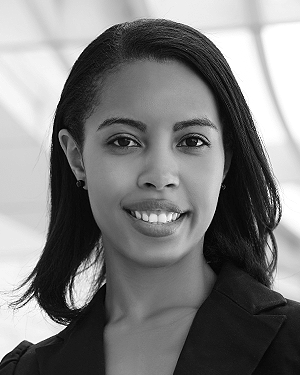
\includegraphics[width=1in,height=1.25in,clip,keepaspectratio]{a1.png}}]{First A. Author}
received the B.S. and M.S. degrees in Computer Science and Engineering from National Institute of Technology, in 2020 and 2022, respectively. He is currently pursuing the Ph.D. degree in Artificial Intelligence at Premier Research Institute. His primary research interests include autonomous multi-agent systems, complex network emergence, distributed algorithmic reasoning, and fault-tolerant foundation model architectures. He has served as a reviewer for leading international conferences and journals in machine learning and autonomous systems.
\end{IEEEbiography}

\begin{IEEEbiography}[{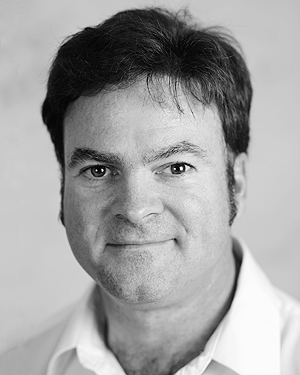
\includegraphics[width=1in,height=1.25in,clip,keepaspectratio]{a2.png}}]{Second B. Author}
received the M.S. and Ph.D. degrees in Electrical and Computer Engineering from Technological University in 2016 and 2020, respectively. She is currently an Associate Professor with the Department of Artificial Intelligence at Technological University. Her research spans natural language processing, collective intelligence, multi-agent reinforcement learning, and neuro-symbolic reasoning. Dr. Author is an active member of the IEEE Computer Society and has published extensively in premier artificial intelligence venues.
\end{IEEEbiography}

\begin{IEEEbiography}[{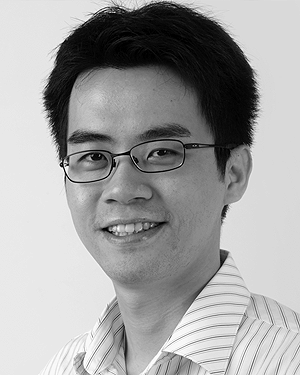
\includegraphics[width=1in,height=1.25in,clip,keepaspectratio]{a3.png}}]{Third C. Author}
(Member, IEEE) received the Ph.D. degree in Computer Science from the National Research Center in 2014. He is currently a Principal Research Scientist with the Department of Information Technology at National Research Center. His research interests encompass distributed systems, large language model scalability, organizational emergence, and Byzantine fault tolerance. He has authored over 60 journal and conference publications and serves on several IEEE Technical Committees.
\end{IEEEbiography}

\EOD

\end{document}
